\lstset{
    language=Python,
    basicstyle=\ttfamily\small,
    keywordstyle=\color{blue},
    stringstyle=\color{red},
    commentstyle=\color{green!50!black},
    numbers=left,
    numberstyle=\tiny\color{gray},
    stepnumber=1,
    showstringspaces=false,
    breaklines=true,
    frame=single,
    captionpos=b,
    tabsize=4,
    literate={á}{{\'a}}1 {â}{{\^a}}1 {ã}{{\~a}}1 {é}{{\'e}}1 {ê}{{\^e}}1 {í}{{\'i}}1 {ó}{{\'o}}1 {ô}{{\^o}}1 {õ}{{\~o}}1 {ú}{{\'u}}1 {ç}{{\c{c}}}1
}

\chapter[Execução da Pesquisa e Análise dos Resultados]{Execução da Pesquisa e Análise dos Resultados} 

Antes de começar a "Execução da Pesquisa e Análise dos Resultados", é crucial enfatizar que todas as fases deste estudo foram realizadas de acordo com as normas éticas e legais pertinentes à investigação científica. Os dados utilizados neste estudo foram obtidos por meio do especialista em Reprodução Humana Assistida, Dr. Bruno Ramalho, e de suas pacientes, que autorizaram o uso dessas informações para fins de pesquisa. As informações foram coletadas na clínica Bruno Ramalho Reprodução Humana, bem como na clínica Genesis, onde o Dr. Bruno também atua. A documentação que comprova isso está devidamente incluída nos anexos deste estudo, incluindo os seguintes documentos essenciais:
\begin{itemize}
  \item \textbf{Parecer da Plataforma Brasil}: Inclui a permissão ética que valida a utilização dos dados dos embriões para a execução deste estudo, garantindo a conformidade com os padrões éticos definidos para pesquisas que envolvem seres humanos (disponível no Anexo \ref{anexo:parecer-cep})
  \item \textbf{Contrato de Autorização para Utilização de Dados em Pesquisa}: Assinado pelo Dr. Bruno Ramalho, que autoriza o uso dos dados clínicos de suas pacientes, essenciais para a modelagem e análise realizadas durante esta pesquisa (disponível no Anexo \ref{anexo:contrato-autorizacao})
  \item \textbf{Termo de Consentimento para Utilização de Dados de Entrevistas, Gravação de Reuniões e Uso de Gravação}: Contrato que permite o uso de discursos, dados e gravações provenientes das reuniões e entrevistas conduzidas com o Dr. Bruno Ramalho, garantindo que as informações e contribuições fornecidas por ele fossem utilizadas com total autorização (disponível no Anexo \ref{anexo:termo-consentimento}).
\end{itemize}
Estes documentos evidenciam o comprometimento ético e a transparência desta pesquisa, enfatizando que todas as informações empregadas foram obtidas de maneira responsável e autorizada.
Os códigos mencionados nas atividades estão disponíveis no repositório do projeto no GitHub, podendo ser acessado aqui: \textbf{\href{https://github.com/sabrinaberno/TCC1}{GitHub-TCC}}, onde são detalhadamente explicados, incluindo a lógica utilizada para sua implementação e os resultados obtidos.
 
\section{Fase 1: Análise e Preparação de Dados}
\subsection{OE1 - Expandir, Processar e Analisar os Dados para Predição de Ploidia}
\subsubsection{Atividade 1 (A1): Análise, Revisão, Seleção e Limpeza de Variáveis para Predição de Euploidia}
O desenvolvimento desta atividade teve início com a verificação da relevância das variáveis com base nos estudos da fundamentação teórica. Esse processo envolveu a análise das variáveis presentes na tabela de dados que serão utilizadas nesta pesquisa, garantindo sua adequação ao objetivo do estudo. 

% As variáveis selecionadas inicialmente são:

% \begin{table}[ht]
%   \begin{tabular}{|l|c|}
%   \hline
%   \textbf{Variáveis} & \textbf{Definição} \\ \hline
%   Id & Identificador numérico de cada paciente. \\ \hline
%   Idade & Idade da paciente no momento do procedimento. \\ \hline
%   Data da biopsia & Data em que foi realizada a biópsia embrionária. \\ \hline
%   Embrião n. & Identificação numérica do embrião dentro do ciclo de fertilização. \\ \hline
%   Estágio & Dia de evolução no cultivo. \\ \hline
%   Morfo & Classificação morfológica dos embriões baseada no estágio de expansão da blástula, estágio inicial do desenvolvimento embrionário. \\ \hline
%   Kidscore & Algoritmo que combina variáveis morfocinéticas e parâmetros de desenvolvimento embrionário. \\ \hline
%   st2 & Primeiro indício de movimentos citoplasmáticos antes da primeira citocinese. \\ \hline
%   t2 & Tempo para 2 células. \\ \hline
%   t3 & Tempo para 3 células. \\ \hline
%   t4 & Tempo para 4 células. \\ \hline
%   t5 & Tempo para 5 células. \\ \hline
%   t8 & Tempo para 8 células. \\ \hline
%   tSC & Tempo de formação do estágio de clivagem sincronizada (Time to Synchronized Compaction). \\ \hline
%   tSB & Tempo para o início da blastulação (Time to Start Blastulation). \\ \hline
%   tB & Tempo para o Blastocisto (Time to Blastocyst). \\ \hline
%   t2-st2 & Intervalo de tempo entre o T2 e o ST2. \\ \hline
%   cc2 (t3-t2) & Tempo necessário para que o embrião passe da divisão de 2 células (T2) para a divisão de 3 células (T3). \\ \hline
%   cc3 (t5-t3) & Tempo necessário para que o embrião passe da divisão de 3 células (T3) para a divisão de 5 células (T5). \\ \hline
%   t5-t2 & Intervalo de tempo entre o estágio de 2 células (T2) e o estágio de 5 células (T5). \\ \hline
%   s2 (t4-t3) & Intervalo de tempo necessário para que o embrião passe do estágio de 3 células (T3) para o estágio de 4 células (T4). \\ \hline
%   s3 (t8-t5) & Intervalo de tempo necessário para que o embrião passe do estágio de 5 células (T5) para o estágio de 8 células (T8). \\ \hline
%   tSC-t8 & Intervalo de tempo entre o estágio em que o embrião atinge a compactação inicial (tSC) e o estágio de 8 células (T8). \\ \hline
%   tB-tSB & Intervalo de tempo entre o estágio em que o embrião atinge o blastocisto inicial (tSB) e o estágio de blastocisto expandido (tB). \\ \hline
%   Ploidia & Estado de ploidia do embrião. \\ \hline
%   \end{tabular}
%   \caption{Variáveis analisadas no modelo de IA para predição de euploidia embrionária. A explicação mais detalhada sobre essas variáveis está no APÊNDICE A}
%   \label{tab:definicoes_variaveis}
% \end{table}

A partir da revisão bibliográfica, conduzimos um processo de seleção das variáveis mais relevantes para o nosso modelo de Inteligência Artificial, fundamentado em evidências científicas. Dessa forma, foi possível identificar um conjunto de variáveis da base de dados que apresentam respaldo teórico quanto à sua influência na evolução do modelo. As variáveis selecionadas para o estudo são: \textbf{Idade, t2, t3, t4, t5, t8, s2, cc2 (t3-t2), tSC, tSB, tB, cc3 (t5-t3), s3 (t8-t5), t5-t2, tSC-t8, tB-tSB, Estágio, Morfo e KIDScore}.

A coluna de \textbf{Plodia} também foi selecionada, pois nos possibilita agrupar os embriões em duas categorias claras, distinguindo entre aqueles com euploidia normal e aqueles com alterações cromossômicas, o que é crucial para a elaboração de um modelo sólido.

Não identificamos estudos que estabelecem uma ligação direta entre o parâmetro \textbf{st2} e a previsão de euploidia. Apesar do movimento citoplasmático antes da citocinese ser um marco significativo no desenvolvimento embrionário, a ausência de provas científicas que liguem esse movimento à qualidade do embrião e à euploidia nos levou a remover o \textbf{st2} da lista de variáveis para o modelo. Igualmente, não foram identificados estudos que analisassem especificamente o intervalo entre \textbf{t2} (o instante em que o embrião alcança a fase de duas células) e \textbf{st2} (movimento citoplasmático pré-citocinese) para prever a euploidia. Como \textbf{st2} foi eliminada, também removemos o parâmetro \textbf{t2-st2} do nosso grupo de variáveis.

A partir disso, conseguimos determinar quais variáveis são fundamentais para a elaboração do nosso modelo de previsão de euploidia. As colunas \textbf{Id, Data da biópsia e Embrião n.} também foram eliminadas, uma vez que não contribuem para o valor do modelo. Portanto, a planilha revisada inclui somente as variáveis que possuem uma ligação comprovada com a previsão de euploidia, fundamentada nas evidências científicas revisadas.

\subsubsection{Limpeza dos Dados}
Ao lidar com os dados ausentes, utilizamos o método de Análise de Casos Completos (ACC), que envolve a remoção de observações que possuem pelo menos um valor ausente (Camargos, 2011). Este procedimento é frequentemente empregado quando o número de dados ausentes é reduzido, assegurando que a remoção de algumas observações não interfira de forma significativa na análise estatística e preserva a consistência do modelo (Camargos, 2011). Em nosso cenário, por se tratar de uma base de dados pequena, optamos por excluir manualmente as linhas com valores ausentes. Essa abordagem foi escolhida por ser mais prática e eficiente, considerando o tamanho reduzido da amostra. Após essa etapa, a planilha foi ajustada com apenas os dados completos.

\subsubsection{Atividade 2 (A2): Normalização dos Dados para Otimização}
A etapa de normalização dos dados é um passo fundamental na criação de modelos de aprendizado de máquina, particularmente em situações onde as variáveis têm diferentes escalas e distribuições. Esta tarefa foi executada com o uso do método Z-Score. Esta metodologia modifica os dados de forma que cada variável possua uma média de 0 e um desvio padrão de 1, explicado na APÊNDICE \ref{apendice:zscore}. 

Antes da aplicação da normalização por Z-Score, foi necessário realizar o pré-processamento dos dados para garantir que todas as variáveis relevantes estivessem em formato numérico. Essa etapa é fundamental em pipelines de aprendizado de máquina, uma vez que a maioria dos algoritmos não consegue operar diretamente com dados categóricos ou textuais. 

\begin{enumerate}
    \item \textbf{Conversão da variável alvo “Ploidia”:} A coluna \texttt{Ploidia}, originalmente categórica com os valores “Euplóide” e “Aneuplóide”, foi convertida para valores binários (0 e 1, respectivamente). Essa codificação binária é necessária para que o modelo classificador interprete corretamente a variável-alvo.
    
    \item \textbf{Transformação da coluna “Estágio”:} A coluna \texttt{Estágio}, que indicava o dia de desenvolvimento embrionário com um prefixo textual (“D3”, “D5”, etc.), teve a letra “D” removida com a função \texttt{str.replace()}, deixando apenas o valor numérico correspondente ao dia. Em seguida, os valores foram convertidos para o tipo \texttt{int} com a função \texttt{pd.to\_numeric()}, assegurando a correta tipagem para análise quantitativa.
    
    \item \textbf{Conversão da classificação morfológica (“Morfo”):} Essa coluna originalmente armazenava uma combinação alfanumérica representando o estágio morfológico do blastocisto (ex: “4AA”, “3BB”). Para torná-la compatível com os modelos, foi criada uma função chamada \texttt{classificar\_morfo()} que categoriza os embriões em quatro grupos (1 a 4), com base na qualidade morfológica indicada no Capítulo 2.
    
    \item \textbf{Extração das colunas numéricas:} Após as transformações, foi extraído um subconjunto contendo apenas colunas numéricas por meio da função \texttt{select\_dtypes()}. Isso assegura que o arquivo de saída contenha apenas dados prontos para normalização e posterior uso em modelos de aprendizado de máquina.
    
    \item \textbf{Exportação do conjunto processado:} Os dados finalizados foram exportados para uma nova planilha Excel, chamada “\texttt{PlanilhaNumerica.xlsx}”, por meio do método \texttt{to\_excel()}, permitindo seu uso direto nas etapas posteriores do pipeline de modelagem.
\end{enumerate}

Seguindo para a normalização, ela foi conduzida com Python e a biblioteca Pandas. O procedimento foi automatizado para simplificar a análise A normalização foi conduzida utilizando a linguagem Python e a biblioteca \texttt{Pandas}, com foco na automação do processo para aplicação em larga escala aos dados morfocinéticos dos embriões. A transformação foi aplicada especificamente às variáveis numéricas previamente selecionadas na fase de escolha de atributos, de forma a garantir consistência na entrada do modelo.

A sequência de passos executados pelo código para a normalização dos dados foi:

\begin{enumerate}
    \item \textbf{Análise dos Dados:} Os dados foram inicialmente importados do arquivo Excel que possui os dados dos embriões, usando a função \texttt{pd.read\_excel()}.
    
    \item \textbf{Identificação das Colunas Numéricas:} Foi aplicada uma função para identificar automaticamente as colunas do tipo numérico. Em seguida, a variável-alvo “\texttt{Ploidia}” foi removida da lista, já que não deve passar pelo processo de normalização.
    
    \item \textbf{Cálculo da Média e Desvio Padrão:} Para cada variável numérica, a média e o desvio padrão foram calculados.
    
    \item \textbf{Utilização do Z-Score:} Para cada valor de uma variável, a média é subtraída e o desvio padrão é dividido, de acordo com a fórmula. Isso modifica os dados para que todas as variáveis apresentem média zero e desvio padrão igual a 1.
    
    \item \textbf{Armazenamento dos Dados Normalizados:} Depois de aplicar o Z-Score, os dados normalizados foram guardados em uma nova planilha Excel, denominada “\texttt{Planilha\_normalizada.xlsx}”.
\end{enumerate}

A escolha do método Z-Score justifica-se por sua capacidade de padronizar variáveis com distribuições distintas, facilitando a convergência de algoritmos de aprendizado de máquina e aumentando a comparabilidade entre atributos \cite{jaiswal2024}. Além disso, essa padronização é especialmente recomendada em modelos que são sensíveis à escala dos dados, como Redes Neurais Artificiais e Máquinas de Vetores de Suporte (SVM). Ao final do processo, o conjunto de dados normalizado encontra-se adequado para ser utilizado nas etapas seguintes do pipeline de modelagem.

\subsection*{Análise da Planilha Normalizada}
Depois de realizar a normalização, a Tabela \ref{tab:normalizacao} gerada apresenta os dados convertidos para que cada variável possua uma média de 0 e um desvio padrão de 1. 

\begin{table}[h!]
  \centering
  \renewcommand{\arraystretch}{1.2} 
  \captionsetup{font=footnotesize, justification=centering, labelsep=period, position=above}
  \caption{Planilha Normalizada}
  \label{tab:normalizacao}
  \begin{tabular}{|c|c|c|c|}
      \vspace{0.2cm} \cellcolor[HTML]{008940}  \textbf{Kidscore} & \cellcolor[HTML]{008940} \textbf{t2} & \cellcolor[HTML]{008940}  \textbf{t3} & \cellcolor[HTML]{008940}  \textbf{t4} \\
      
      \hline
      -0,1651468441 & -1,04331772 & -0,2061446738 & -0,1365241993 \\
      -0,3621219891 & 0,0828611265 & 0,1102377935 & -0,04951654895 \\
      1,509141888 & -0,7805426557 & -0,4547308981 & -0,8035828516 \\
      -0,1651468441 & 0,233018306 & 0,08769304581 & -0,1365241993 \\
      1,75536082 & -0,4426890018 & -0,4095334028 & -0,8909505013 \\
      1,410654316 & -0,9306998352 & -0,6129221317 & -1,151613453 \\
      0,8689726671 & -1,231014194 & -0,5677246364 & -1,064605802 \\
      -0,3128782029 & -0,8180819506 & -0,4547308981 & -0,7745803015 \\
      0,9182164534 & -1,11839631 & -0,9067058513 & -1,586651704 \\
      -0,06665927163 & 0,833647024 & 0,607410242 & 0,7625458359 \\
      -0,5095833479 & 0,833647024 & 1,217576429 & 1,197593105 \\
      -1,888679363 & 0,3831754855 & 0,0650429815 & -0,07851909905 \\
      \hline
  \end{tabular}
  \caption*{\scriptsize Fonte: Autoras (2024)}
\end{table}
\FloatBarrier

Isso reduz o efeito das variações de escala entre as variáveis e simplifica a compreensão dos dados. A tabela normalizada foi verificada e todos os valores foram ajustados de acordo com a fórmula do Z-Score, com a média e o desvio padrão calculados para cada linha. Por exemplo, a variável "t2" tinha valores que oscilavam entre 19 e 38 horas antes da normalização, indicando uma ampla dispersão na faixa de dados. Depois de normalizados, os dados da variável foram convertidos em uma escala com média zero e desvio padrão de 1. Isso permitiu que todos os valores da variável estivessem comparáveis, mesmo com a grande variação original.

\subsection*{Efeito da Normalização na Comparabilidade das Variáveis}
O principal benefício de normalizar as variáveis é que agora é possível compará-las de forma mais justa. Antes da normalização, variáveis como o "t8" (que apresentava uma amplitude maior) poderiam impactar de forma desproporcional o modelo de aprendizado de máquina, enquanto variáveis como o "t2", com uma amplitude menor, poderiam ser desconsideradas. Com a normalização, todas as variáveis estão na mesma escala, possibilitando uma avaliação justa de cada uma durante o treinamento do modelo.

Este efeito é especialmente relevante em algoritmos que lidam com escalas de variáveis, como as redes neurais. Com os dados normalizados, as conexões entre as variáveis podem ser examinadas de forma mais nítida, simplificando a elaboração de modelos preditivos mais confiáveis.

\subsubsection{Atividade 3 (A3): Identificação da Correlação entre os Parâmetros na Previsão da Ploidia do Embrião}

Após os dados estarem normaizados, iniciamos a utilização do coeficiente de \textbf{correlação de Spearman}, explicado no APÊNDICE \ref{apendice:spearman}, que foi escolhido para esta atividade devido à necessidade de reconhecer relações entre os parâmetros documentados nos dados dos embriões e a porcentagem de euploidia. A metodologia leva em conta a classificação ordinal das observações, minimizando os efeitos de valores atípicos e permitindo a análise de variáveis com distribuições não normais \cite{sousa2019}.

O programa em Python criado para essa análise foi desenvolvido para ser modular, eficaz e gerar resultados claros tanto em formato visual quanto textual. Ele emprega as bibliotecas \textit{Pandas, SciPy, Matplotlib e python-docx} para manipular dados, determinar correlações, produzir gráficos e elaborar relatórios em Word. A seguir, detalha-se a lógica do código:

\begin{itemize}
    \item \textbf{Carregamento e Preparação dos Dados}: As informações dos embriões foram processadas a partir da Planilha de Dados Refinada, utilizando todas as colunas disponíveis. Essa etapa garante que todas as variáveis relevantes sejam consideradas.
    \item \textbf{Cálculo da Correlação de Spearman}: O coeficiente de Spearman foi calculado para todas as combinações possíveis de variáveis, utilizando a função \texttt{spearmanr} da biblioteca SciPy. O método \texttt{"omit"} foi empregado para lidar com valores ausentes, garantindo maior robustez mesmo que não existam dados faltantes nesta planilha.
    \item \textbf{Criação de Gráficos de Dispersão}: Para cada par de variáveis, foram criados gráficos de dispersão que auxiliam na análise numérica e permitem a identificação visual de padrões. As cores foram padronizadas, com a variável 1 (\texttt{var1}) em verde claro e marcador ``o'', e a variável 2 (\texttt{var2}) em azul escuro e marcador ``x''.
    \item \textbf{Elaboração de Relatório Automatizado}: O relatório gerado contém descrições textuais dos coeficientes e gráficos correspondentes. Este documento automatizado facilita a comunicação visual e escrita dos resultados.
\end{itemize}

O código analisa a correlação entre as variáveis numéricas em uma sequência de dados, empregando o coeficiente de Spearman. Ele inicia carregando a planilha Excel com as informações dos embriões e seleciona todas as colunas relevantes para a análise. O coeficiente de Spearman é calculado para cada par de variáveis, avaliando a intensidade e a direção da relação monótona entre elas. Os resultados são armazenados em um \texttt{DataFrame}, que é uma estrutura de dados bidimensional do Pandas, semelhante a uma tabela, permitindo fácil manipulação e análise. Esta tabela é então exportada para um arquivo Excel chamado \texttt{correlation\_results.xlsx}.

Após isso, o programa gera gráficos de dispersão para observar as correlações, ressaltando os padrões das variáveis associadas. Esses gráficos, juntamente com os coeficientes de correlação, são automaticamente incorporados a um documento Word. No final, temos um relatório completo com as análises e visualizações, salvo como um arquivo chamado \texttt{relatorio\_correlacoes.docx}, que contém todos os gráficos de dispersão para as combinações examinadas e valores de correlação relacionados. 

Em seguida, apresentaremos a avaliação dos resultados mais relevantes obtidos a partir dos dois documentos gerados pelo código, destacando as variáveis com correlações mais significativas, bem como aquelas com pouca ou nenhuma interação. Para uma visão mais abrangente dos dados, a matriz de correlação entre todas as variáveis está disponível no Anexo \ref{anexo:correlacoes}.

\subsection*{Idade}
A correlação com \textbf{t4 (-0,15) sugere que a idade exerce uma influência negativa leve sobre eventos específicos do desenvolvimento embrionário}. Mulheres mais velhas podem apresentar embriões com ligeiro atraso no tempo necessário para atingir o estágio \textit{t4}. Em relação ao tempo para 5 células, \textit{t5} (0.11), obteve uma correlação positiva.\textbf{ Isso sugere uma tendência muito sutil de que embriões em fases mais avançadas estejam ligados a mães de mais idade}.

\begin{figure}[h]
    \captionsetup{font=footnotesize, justification=centering, labelsep=period, position=above}
    \caption{Dispersão entre Idade e t4 - Coeficiente de Spearman: -0.15 e entre Idade e t5 - Coeficiente de Spearman: 0.11}
    \label{fig:idade-t4-t5}
    \centering
    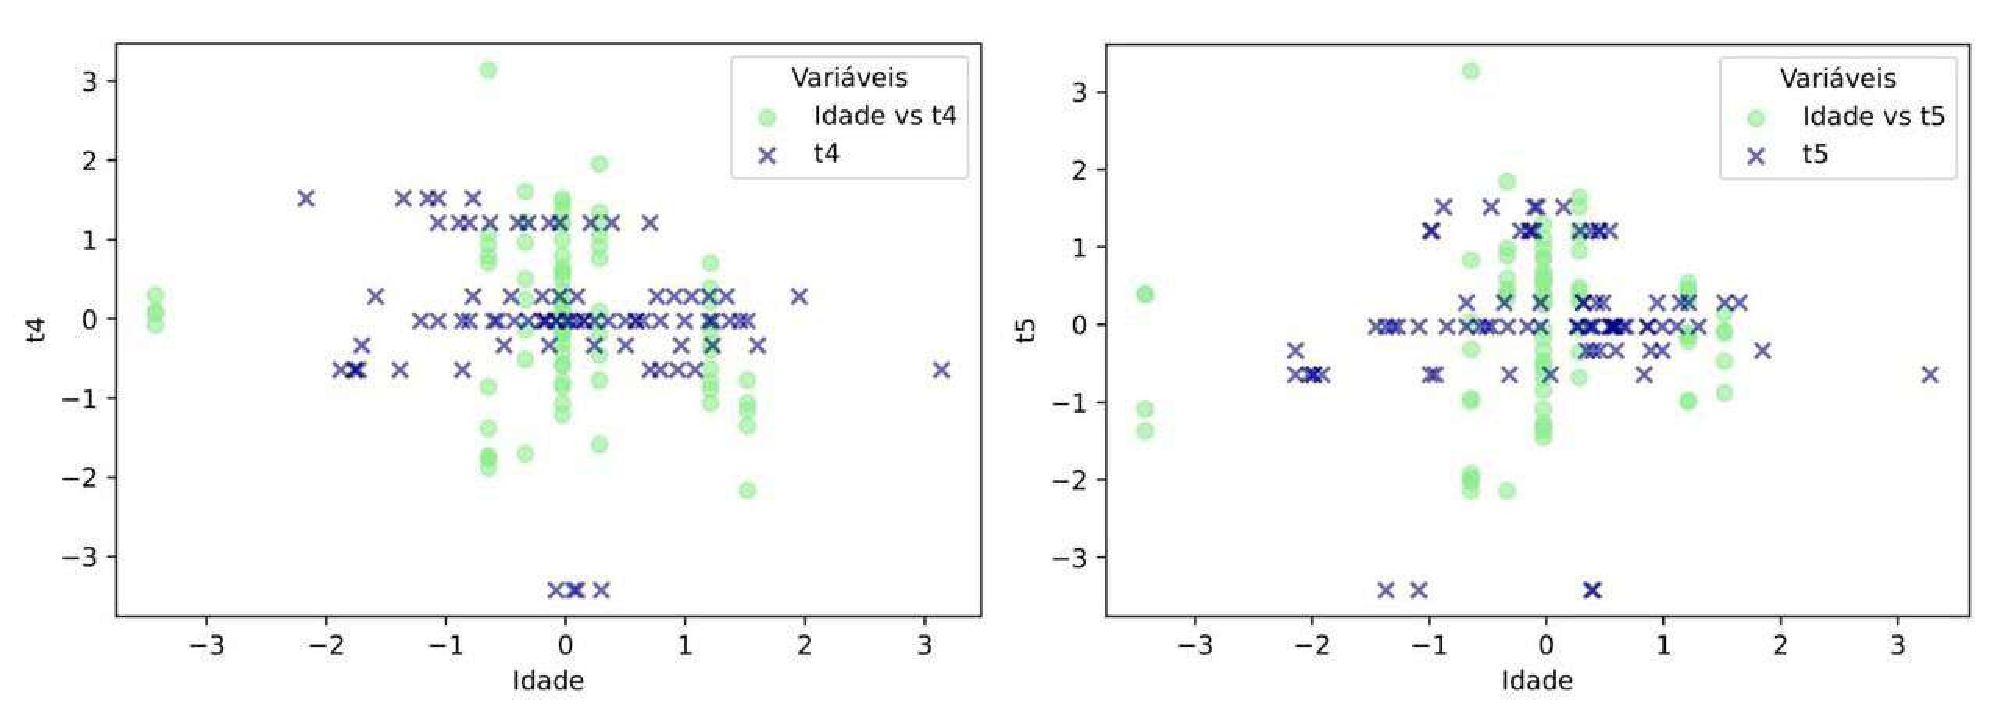
\includegraphics[scale=0.4]{figuras/Spearman/idade-t4-t5.pdf}
    \vspace{0.3cm} 
    % \caption{A análise da dispersão entre Idade e as variáveis t4 e t5, utilizando o coeficiente de Spearman, revela correlações leves. O coeficiente de Spearman entre Idade e t4 foi de -0,15, indicando uma correlação monotônica negativa fraca, ou seja, à medida que a idade aumenta, há uma leve tendência de redução no tempo t4. Já entre Idade e t5, o coeficiente foi de 0,11, sugerindo uma correlação monotônica positiva fraca, indicando que o aumento da idade pode estar associado a um leve aumento no tempo t5.}
    \begin{minipage}{\linewidth}
        \centering
    \end{minipage}
\end{figure}
\FloatBarrier 

Ao reparar em alguns índices negativos, observamos os índices \textbf{tSB (-0.10), cc2 (t3-t2) (-0.17), s2 (t4-t3) (-0.24),  s3 (t8-t5) (-0.28) e a Ploidia(-0.50)}. Nota-se que os coeficientes mais próximos de 0 (como -0,10 a -0,28) indicam uma correlação negativa fraca. Isso traduz que há uma tendência muito sutil de que, quando uma variável aumenta, a idade, a outra diminui. Em \textit{tSB} Figura \ref{fig:idade-tSB-cc2-s2-s3}, o coeficiente negativo insinua que o tempo de formação inicial da blastocisto tende a ser menor em embriões provenientes de mães mais velhas. Na variável \textit{cc2}, Figura \ref{fig:idade-tSB-cc2-s2-s3}, a correlação desfavorável sugere uma maior irregularidade no intervalo entre a segunda e a terceira divisão celular (t2 para t3) em embriões de mães mais velhas. Em \textbf{s2} (Figura \ref{fig:idade-tSB-cc2-s2-s3}) e \textit{s3} (Figura \ref{fig:idade-tSB-cc2-s2-s3}), mostra que a idade materna também está ligada a uma diminuição na eficácia do intervalo entre as divisões celulares de t3 para t4. Isso indica um efeito na fase intermediária do ciclo celular. Nos embriões de mães mais velhas, o período entre a fase de 8 células e a formação do blastocisto final é estendido, sinalizando obstáculos no progresso dessas fases. Todos esses atrasos podem ser cruciais, já que fases iniciais bem sincronizadas são fundamentais para um desenvolvimento embrionário adequado, mostrando como uma idade avançada pode afetar o desenvolvimento embrionário, afirmando a bibliografia estudada, fato já citado por \citeonline{borges2022}, que reitera que \textbf{a idade materna exerce maior influência sobre a qualidade embrionária}.

\begin{figure}[h]
    \captionsetup{font=footnotesize, justification=centering, labelsep=period, position=above}
    \caption{Dispersão entre Idade e tSB - Coeficiente de Spearman: -0.10 | Dispersão entre Idade e cc2 (t3-t2) - Coeficiente de Spearman: -0.15 | Dispersão entre Idade e s2 (t4-t3) - Coeficiente de Spearman: -0.24 | Dispersão entre Idade e s3 (t8-t5) - Coeficiente de Spearman: -0.28}
    \label{fig:idade-tSB-cc2-s2-s3}
    \centering
    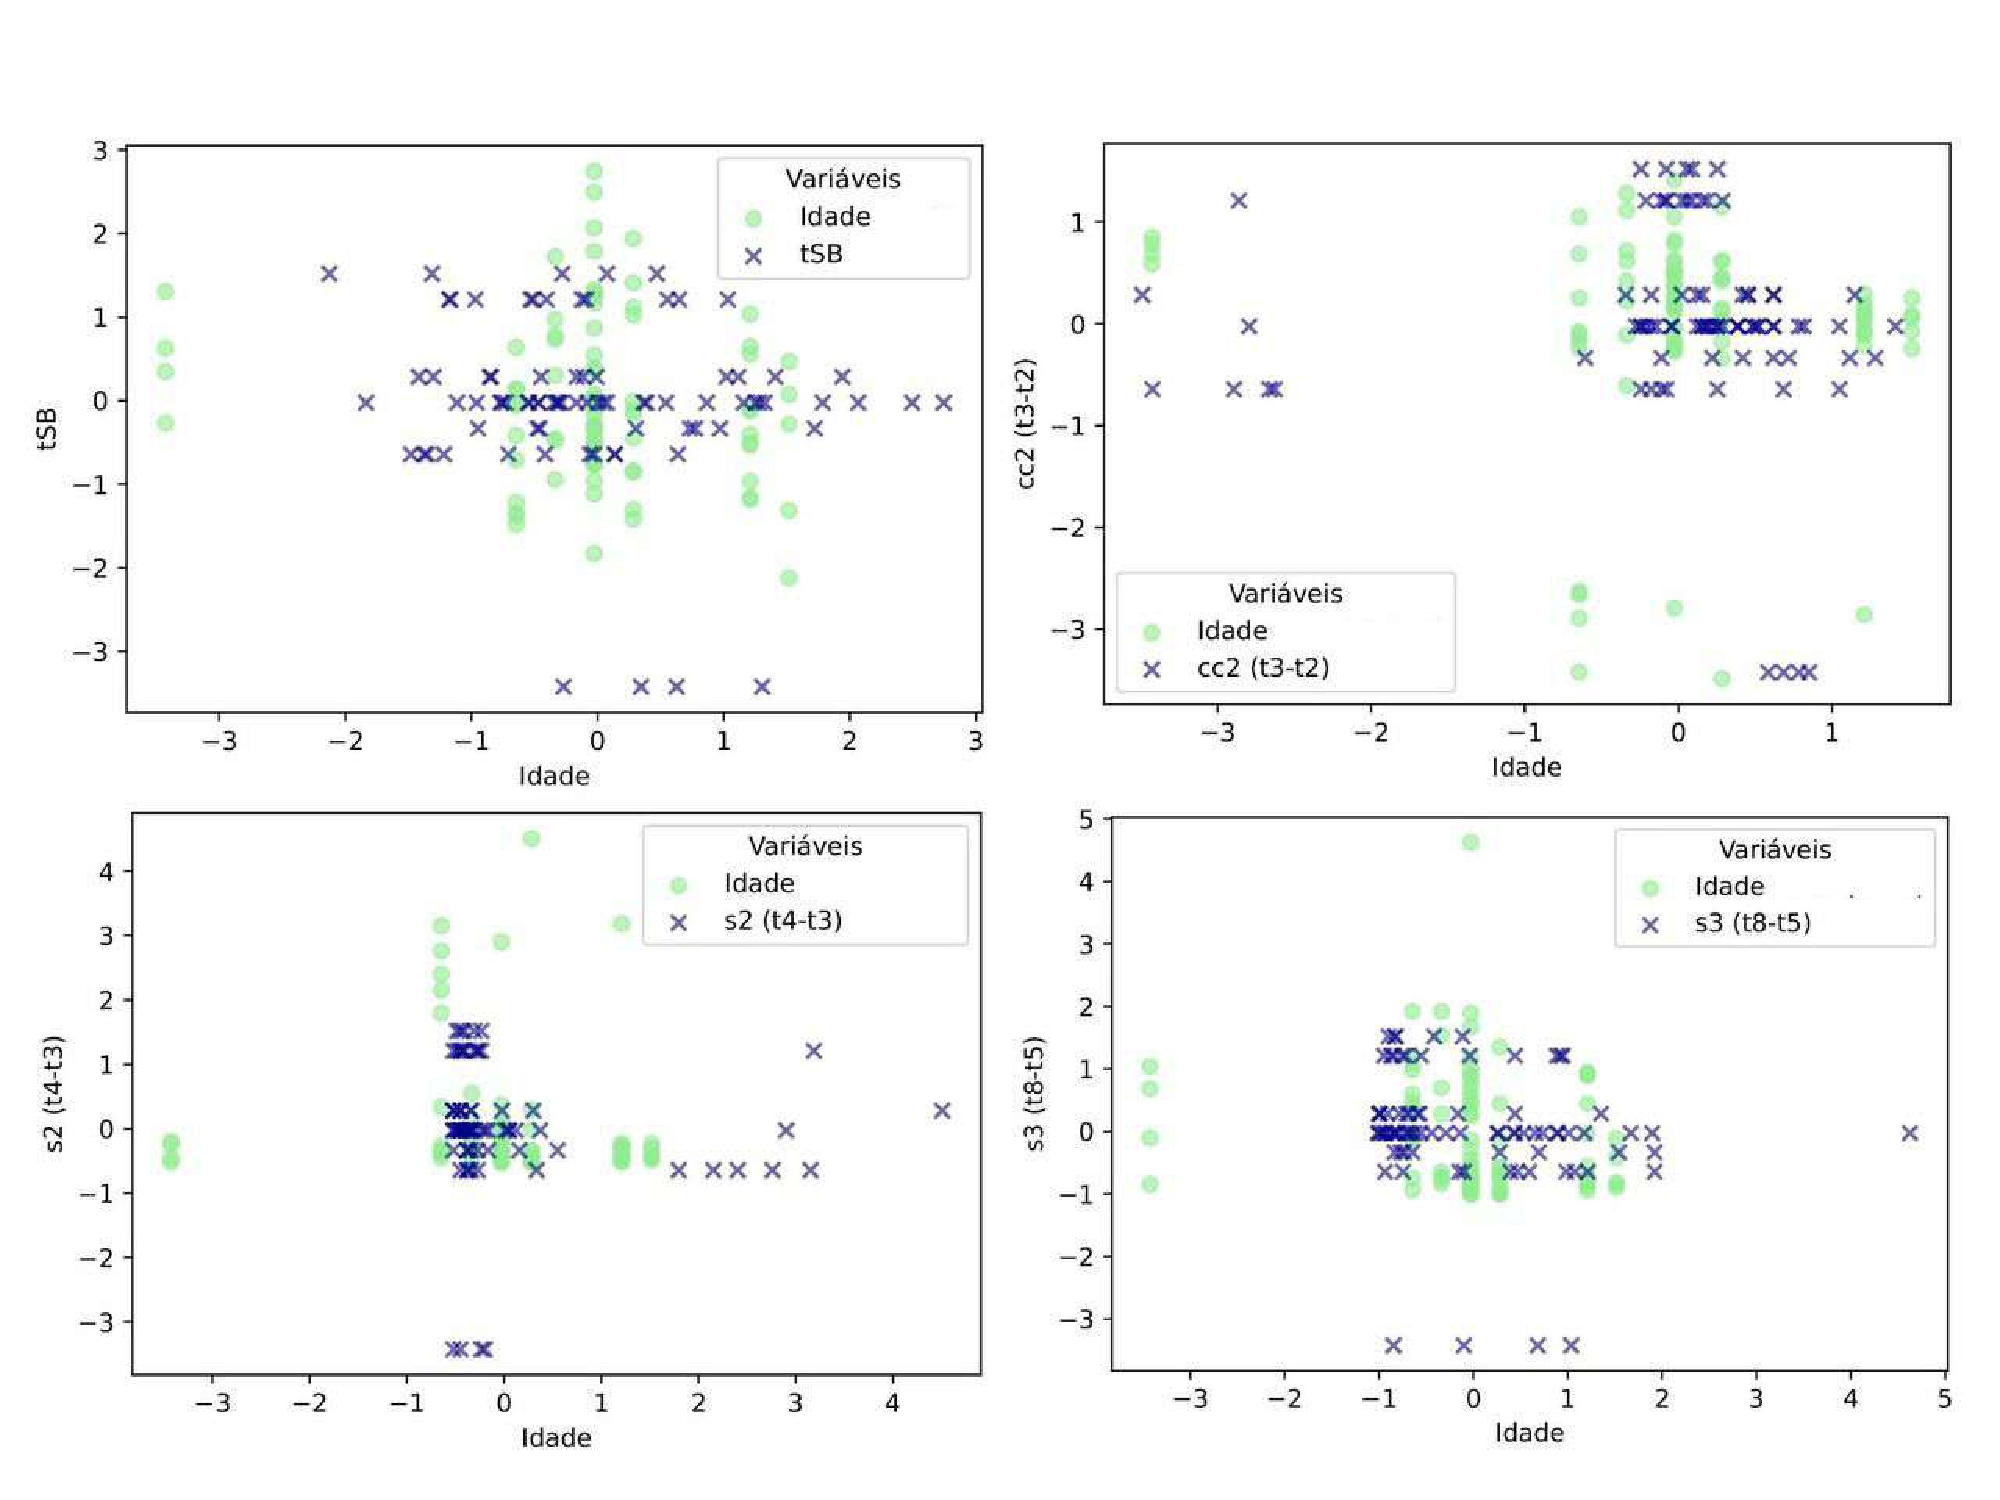
\includegraphics[scale=0.4]{figuras/Spearman/Idade-tSB_cc2_s2_s3.pdf}
    \vspace{0.3cm} 
    % \caption{A análise das relações entre Idade e as variáveis tSB, cc2 (t3-t2), s2 (t4-t3) e s3 (t8-t5) revela correlações negativas de diferentes intensidades, sugerindo que o aumento da idade pode estar associado a uma redução nos respectivos intervalos de tempo. A correlação entre Idade e tSB (-0,10) e entre Idade e cc2 (t3-t2) (-0,15) é fraca, indicando uma leve tendência de diminuição desses valores com o aumento da idade, mas sem um padrão claro. Já a correlação entre Idade e s2 (t4-t3) (-0,24) é moderadamente negativa, sugerindo uma relação mais perceptível entre o aumento da idade e a redução desse intervalo. A relação mais intensa foi observada entre Idade e s3 (t8-t5) (-0,28), apontando que a idade pode influenciar de maneira mais consistente a redução desse tempo. }
    \begin{minipage}{\linewidth}
        \centering
    \end{minipage}
\end{figure}
\FloatBarrier

E por fim temos a \textit{Ploidia (-0,50)}, a correlação negativa mais relevante entre todas as outras variáveis demonstrando que \textbf{a alta idade materna está ligada a uma diminuição na proporção de embriões euploides. Esta informação indica que embriões de mães mais velhas contêm uma proporção reduzida de euploidia, o que pode estar ligado a uma queda na qualidade genética dos embriões}. Portanto, a idade materna é um dos elementos chave na diminuição da euploidia embrionária, alinhando com as informações de \textit{Fertility and Ageing} \cite{eshre2005}, que também reitera que o aumento da aneuploidia em embriões está diretamente associado ao envelhecimento materno.

\subsection*{Estágio}
Os coeficientes de correlação de Spearman entre os \textit{estágios} e os tempos de transição celular \textit{(t2, t3, t4, t5, t8)} revelam relações positivas moderadas. Esses dados indicam que, \textbf{conforme o embrião progride para estágios mais avançados, os tempos associados às divisões celulares iniciais tendem a aumentar de forma sutil}. Esses resultados sugerem que o progresso do estágio embrionário está associado a um padrão de desenvolvimento, possivelmente, mais metódico nos estágios iniciais e intermediários do ciclo celular.

As correlações positivas observadas entre o \textit{estágio} embrionário e os tempos \textit{tSC (0,50), tSB (0,53) e tB (0,59)} indicam uma conexão significativa entre o progresso do estágio embrionário e o desenvolvimento contínuo das estruturas celulares. O incremento nos índices de correlação sugere que, conforme \textbf{o embrião avança para fases mais desenvolvidas, há uma maior regularidade no cumprimento dos marcos temporais dessas transições}. Isso implica que o estágio embrionário atua como um indicador abrangente da qualidade e da evolução do desenvolvimento embrionário.

A relação inversa entre o \textit{estágio} de desenvolvimento e a \textit{ploidia (-0,24)} indica que, \textbf{embora essa correlação seja moderada, sugere que o estágio de desenvolvimento pode ter um impacto negativo na ploidia}. 

\subsection*{Morfo}
A avaliação da variável \textit{Morfo}, que categoriza a expansão morfológica dos embriões em fases iniciais, revelou correlações moderadamente negativas com variáveis temporais como \textbf{t2 (-0.38), t3 (-0.43) e t5 (-0.45)}. Esses achados sugerem que \textbf{embriões com características morfológicas menos expansivas costumam apresentar atrasos nos primeiros tempos de divisão celular}. Dessa forma, os dados estão alinhados com a literatura, que cita que a morfologia do embrião é um fator determinante para o potencial de implantação e a qualidade embrionária \citeonline{capalbo2014}.

Ao examinarmos os intervalos \textit{cc2 (t3-t2) (-0,38) e cc3 (t5-t3) (-0,31)}, os gráficos corroboram essa tendência, destacando que embriões que apresentam alterações morfológicas menos favoráveis quando enfrentam flutuações no ritmo de desenvolvimento celular, a medida que uma variável aumenta, a outra vem a diminuir. Esses resultados enfatizam a relevância de uma divisão celular sincronizada para preservar características morfológicas ideais, evidenciando como o ritmo do ciclo celular influencia diretamente a qualidade estrutural do embrião.

A correlação entre \textit{Morfo} e \textit{Ploidia} exibe um coeficiente de correlação de \textit{0.05}, sugerindo uma ligação positiva, porém extremamente fraca. Isso sugere que, neste conjunto de dados, as características morfológicas dos embriões não parecem estar diretamente ligadas à euploidia. 

\subsection*{t2, t3, t4, t5 e t8}
Existe uma forte interdependência entre os tempos de transição celular, como evidenciado pela correlação de \textit{0.89} entre \textit{t2 e t4}, indicando que esses eventos de desenvolvimento estão fortemente associados, à medida que uma variável aumenta, a outra também aumenta de forma consistente. A correlação entre \textit{t3 e t2 (0.78), t4 e t5 (0.56)} e entre \textit{t5 e t8 (0.52)} também demonstra alinhamento nas fases iniciais e intermediárias do desenvolvimento embrionário. 

\begin{figure}[h]
    \captionsetup{font=footnotesize, justification=centering, labelsep=period, position=above}
    \centering
    \begin{minipage}[b]{0.45\linewidth}
        \caption{Dispersão entre t2 e t4 - Coeficiente de Spearman: 0.89}
        \label{fig:t2-t4}
        \centering
        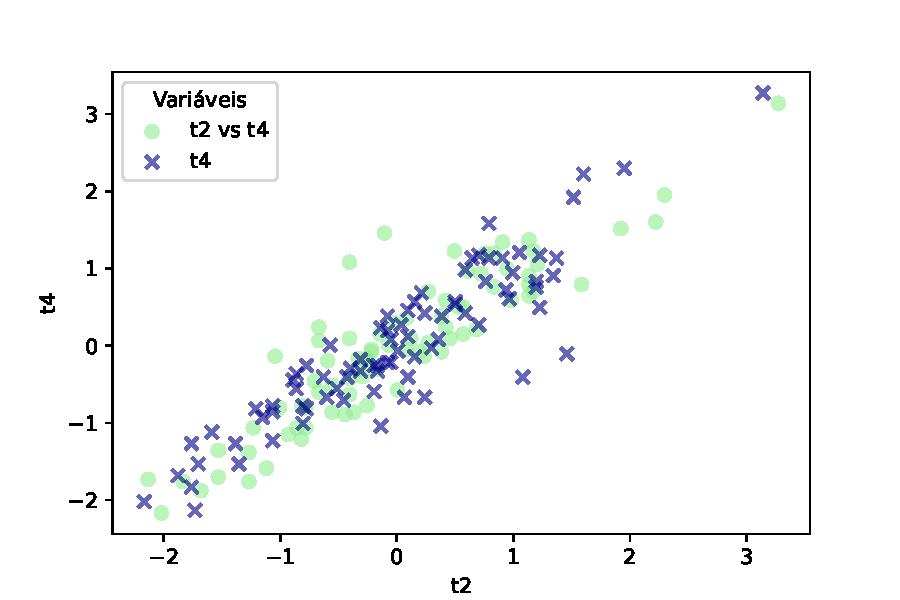
\includegraphics[scale=0.49]{figuras/Spearman/t2-t4.pdf}
        \vspace{0.3cm}
        % \caption{Indica uma correlação monotônica positiva forte. Isso significa que, à medida que o valor de t2 aumenta, t4 também tende a aumentar de forma consistente.}
        \begin{minipage}{\linewidth}
            \centering
        \end{minipage}
    \end{minipage}
    \hspace{0.05\linewidth}
    \begin{minipage}[b]{0.45\linewidth}
        \caption{Dispersão entre t3 e t2 - Coeficiente de Spearman: 0.78}
        \label{fig:t3-t2}
        \centering
        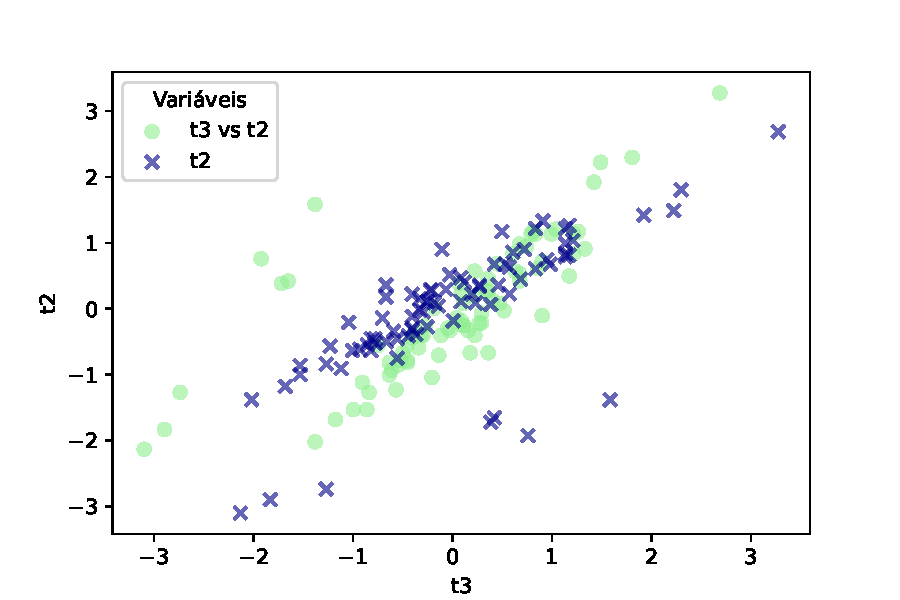
\includegraphics[scale=0.35]{figuras/Spearman/t3-t2.pdf}
        \vspace{0.3cm}
        % \caption{Indica uma correlação monotônica positiva forte. Isso significa que, à medida que t2 aumenta, t3 também tende a aumentar de forma consistente, embora com uma relação um pouco menos intensa do que a observada entre t2 e t4.}
        \begin{minipage}{\linewidth}
            \centering
            \scriptsize{Fonte: Autoras (2025)}
        \end{minipage}
    \end{minipage}
\end{figure}
\FloatBarrier

\begin{figure}[h]
    \captionsetup{font=footnotesize, justification=centering, labelsep=period, position=above}
    \centering
    \begin{minipage}[b]{0.45\linewidth}
        \caption{Dispersão entre t4 e t5 - Coeficiente de Spearman: 0.56}
        \label{fig:t4-t5}
        \centering
        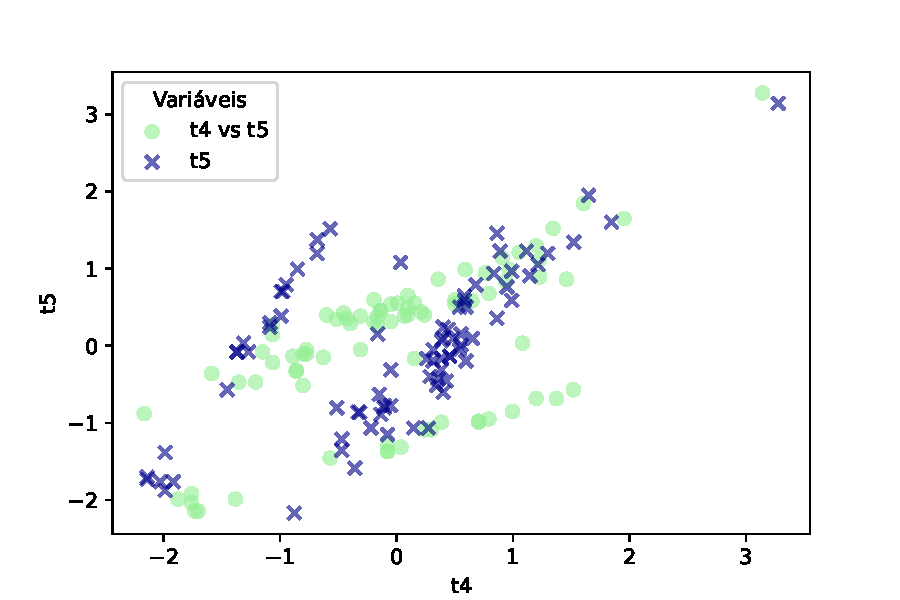
\includegraphics[scale=0.48]{figuras/Spearman/t4-t5.pdf}
        \vspace{0.3cm}
        % \caption{Indica uma correlação monotônica positiva moderada. Isso significa que, à medida que t4 aumenta, t5 também tende a aumentar. Esse resultado sugere que o tempo necessário para atingir t5 está parcialmente influenciado pelo tempo t4}
        \begin{minipage}{\linewidth}
            \centering
        \end{minipage}
    \end{minipage}
    \hspace{0.05\linewidth}
    \begin{minipage}[b]{0.45\linewidth}
        \caption{Dispersão entre t5 e t8 - Coeficiente de Spearman: 0.52}
        \label{fig:t5-t8}
        \centering
        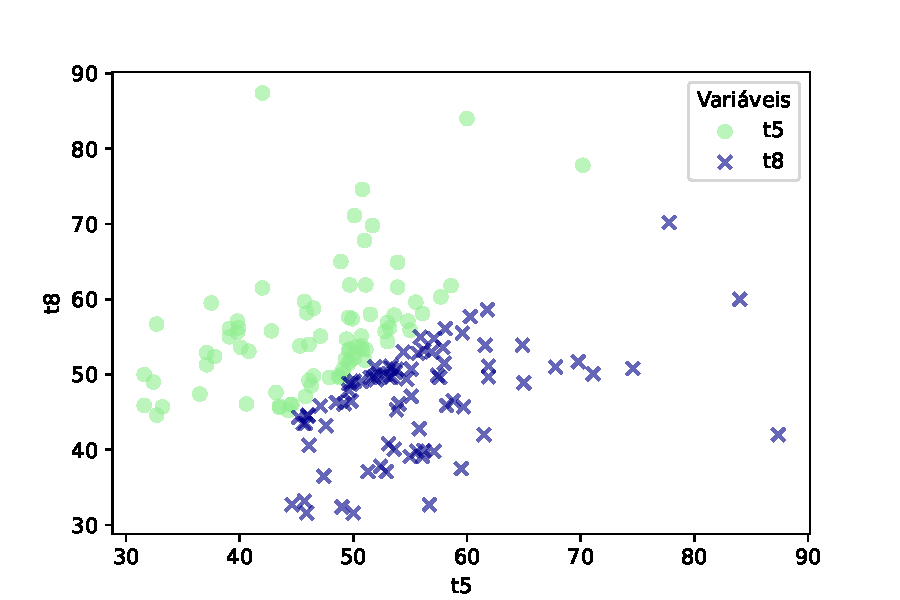
\includegraphics[scale=0.48]{figuras/Spearman/t5-t8.pdf}
        \vspace{0.3cm}
        % \caption{Indica uma correlação monotônica positiva moderada. Isso sugere que, à medida que t5 aumenta, t8 também tende a aumentar. Essa correlação sugere uma dependência entre esses dois tempos}
        \begin{minipage}{\linewidth}
            \centering
        \end{minipage}
    \end{minipage}
\end{figure}
\FloatBarrier

A correlação quase nula entre \textit{t2 (-0.08), t3 (-0.06), t4 (-0.02), t8 (-0.07) e a ploidia}, demonstram uma falta de correlação entre essas variáveis para a determinação de um embrião euploidia ou aneuplóide. Já \textbf{\textit{t5} e \textit{ploidia (-0.24)} indica que atrasos nesse estágio de desenvolvimento, estão ligados a uma qualidade genética inferior (menor ploidia)}, alinhando com a literatura, que destaca t5 como o indicador mais relevante do potencial de implantação \citeonline{cruz2012}. 

\subsection*{tSC}
Ao relacionar a variável de Tempo de formação do estágio de clivagem sincronizada (Time to Synchronized Compaction) com as variáveis de tempos de transição celular, \textit{t2 (0.40), t3 (0.42), t4 (0.43), t5 (0.35) e t8 (0.35)}, indicam uma relação de intensidade moderada e positiva durante o desenvolvimento embrionário, sendo mais acentuada nos estágios iniciais e intermediários. Esses padrões indicam que o \textbf{tSC tem um papel mais significativo nas etapas iniciais e intermediárias do desenvolvimento, diminuindo seu impacto progressivamente conforme o tempo passa}. 

As correlações de \textit{tSC} com \textit{tSB (0.75) e tB (0.74)} demonstram uma forte ligação entre essas variáveis, indicando que estão fortemente conectadas, em que a medida que uma variável aumenta, a outra também aumenta de forma consistente. Isso indica uma relação quase linear, em que mudanças no tSB impactam diretamente no tSC, evidenciando uma ligação funcional direta entre os dois acontecimentos.

\begin{figure}[h]
    \captionsetup{font=footnotesize, justification=centering, labelsep=period, position=above}
    \centering
    \begin{minipage}[b]{0.45\linewidth}
        \caption{Dispersão entre tSC e tSB - Coeficiente de Spearman: 0.75}
        \label{fig:tSC-tSB}
        \centering
        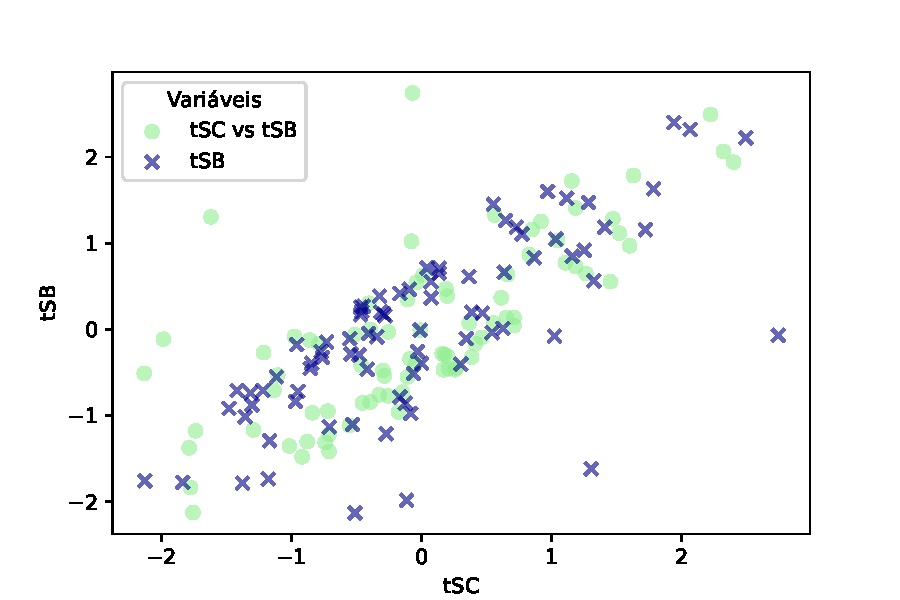
\includegraphics[scale=0.35]{figuras/Spearman/tSC-tSB.pdf}
        \vspace{0.3cm}
        % \caption{A alta correlação entre essas duas variáveis sugere que há uma relação significativa entre elas no desenvolvimento embrionário, indicando que o tempo tSB pode ser um fator importante no comportamento do tempo tSC.}
        \begin{minipage}{\linewidth}
            \centering
            \scriptsize{Fonte: Autoras (2025)}
        \end{minipage}
    \end{minipage}
    \hspace{0.05\linewidth}
    \begin{minipage}[b]{0.45\linewidth}
        \caption{Dispersão entre tSC e tB - Coeficiente de Spearman: 0.74}
        \label{fig:tSC-tB}
        \centering
        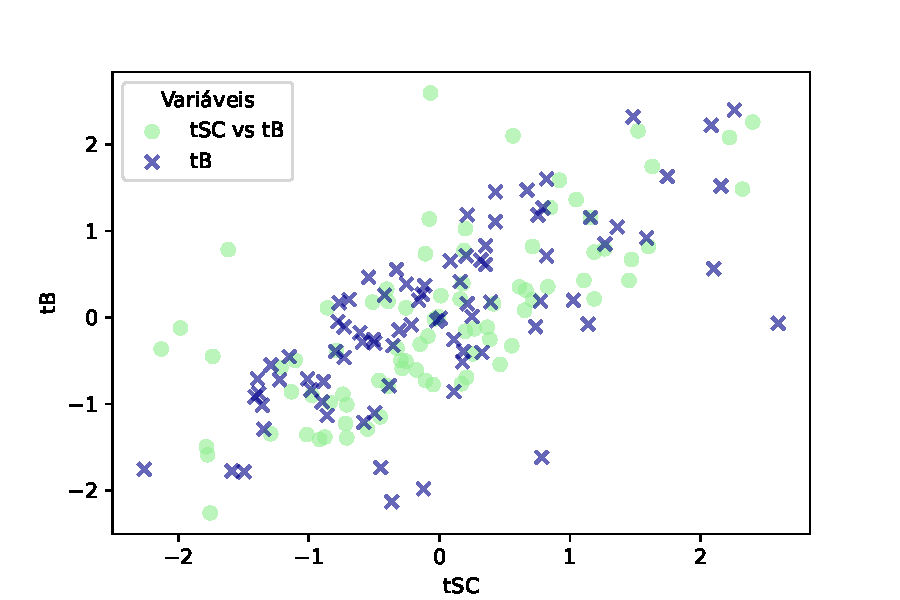
\includegraphics[scale=0.35]{figuras/Spearman/tSC-tB.pdf}
        \vspace{0.3cm}
        % \caption{Há uma tendência clara de que, conforme tB aumenta, tSC também se eleva, sugerindo que essas duas variáveis estão fortemente associadas no contexto do desenvolvimento embrionário. }
        \begin{minipage}{\linewidth}
            \centering
            \scriptsize{Fonte: Autoras (2025)}
        \end{minipage}
    \end{minipage}
\end{figure}
\FloatBarrier

Os coeficientes de correlação de tSC com os intervalos de tempo \textit{cc2 (t3-t2) (0.41), cc3 (t5-t3) (0.24) e t5-t2 (0.34)} apresentam relações positivas que variam de moderadas a fracas, sinalizando variados níveis de concordância com esses tempos acumulados. Estes achados indicam que a influência do tSC se \textbf{reduz} conforme os períodos de tempo se estendem.

Por fim, a correlação com a \textit{Ploidia (-0.04)}, é fraca e negativa, sugerindo que não existe uma conexão relevante entre essas variáveis. Este resultado indica que Ploidia pode estar ligada a processos diferentes que não afetam diretamente \textit{tSC}.

\subsection*{tSB}
Ao analisar sua realção com \textit{t2 (0.43), t3 (0.56), t4 (0.57), t5 (0.39) e t8 (0.40)} mostram relações positivas de intensidade moderada, conforme uma variável aumenta, a outra segue um aumento consistente, aumentando nos estágios iniciais e intermediários e apresentando um ligeiro declínio nos estágios posteriores. A relação com \textit{t2} \textbf{indica que os eventos iniciais exercem um efeito significativo no comportamento de \textbf{tSB}}. A forte ligação com \textit{t3 e t4} indica que \textbf{esses estágios intermediários têm uma influência mais significativa sobre \textbf{tSB}}. Em contrapartida, as correlações moderadas com \textbf{t5 e t8} sugerem uma redução na conexão nos estágios subsequentes, evidenciando um efeito menos significativo de \textit{tSB} conforme os processos progridem no desenvolvimento.

As correlações entre \textit{tSB e tSC (0.75), tB (0.93) e cc2 (t3-t2) (0.63)} evidenciam ligações fortes e relevantes, indicando uma interdependência entre essas variáveis. A forte ligação com \textbf{tSC} sugere que alterações em uma variável têm um \textbf{impacto direto} na outra. \textbf{A correlação com tB indica uma dependência quase total entre as duas variáveis}, indicando que são praticamente comparáveis em termos de sua interação. Ademais, a correlação robusta com cc2 (t3-t2) indica que \textbf{o período entre t3 e t2 tem um impacto considerável sobre tSB, possivelmente por causa do efeito direto dos eventos temporais iniciais no comportamento dessa variável}. O gráfico ilustra a forma que \textit{tSB e tB} possuem uma relação de crescimento mútuo entre si, quase se espelhando. Dessa forma, alterações em tB podem ser significativas para mudanças em tSB.

\begin{figure}[h]
    \captionsetup{font=footnotesize, justification=centering, labelsep=period, position=above}
    \caption{Dispersão entre tSB e tB - Coeficiente de Spearman: 0.93}
    \label{fig:tSB-tB}
    \centering
    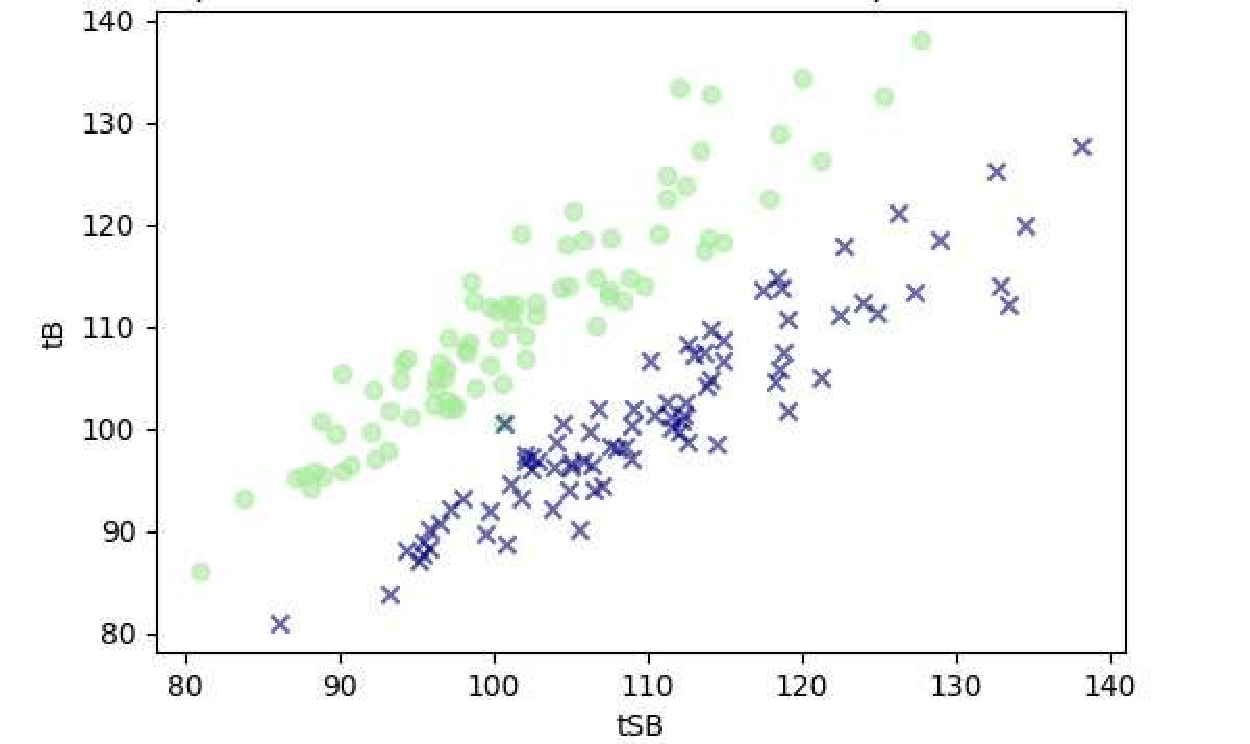
\includegraphics[scale=0.40]{figuras/Spearman/tSB-tB.pdf}
    \vspace{0.3cm} 
    % \caption{A análise da dispersão entre tSB e tB, com um coeficiente de Spearman de 0,93, revela uma correlação positiva extremamente forte. Isso indica que, à medida que tB aumenta, tSB também tende a aumentar de maneira quase perfeitamente sincronizada.}
    \begin{minipage}{\linewidth}
        \centering
    \end{minipage}
\end{figure}
\FloatBarrier

O coeficiente de correlação de \textit{tSB com Ploidia (-0.11)} é fraco e negativo, sugerindo que não existe uma conexão evidente ou relevante entre essas variáveis. Este resultado indica que Ploidia é afetada por elementos diferentes, que não estão diretamente ligados aos processos ligados à tSB.

\subsection*{tB}
As correlações entre \textit{tB} e os tempos de desenvolvimento \textit{t2 (0.40), t3 (0.48), t4 (0.50), t5 (0.35) e t8 (0.37)} exibem relações moderadamente positivas, sugerindo que tB está ligado a eventos temporais durante o ciclo embrionário, sendo mais intensa nos estágios intermediários. 

As correlações de tB com os intervalos de tempo \textit{cc2 (t3-t2) (0.54) e tSC-t8 (0.47)} ressaltam a influência de processos particulares no comportamento dessa variável. A correlação moderada-alta com \textit{cc2 (t3-t2)} indica que \textbf{os períodos de transição entre t3 e t2 têm uma influência relevante no comportamento de tB}, sugerindo que as dinâmicas nos estágios iniciais influenciam diretamente o desenvolvimento subsequente. Em contrapartida, a correlação moderada entre \textit{tSC e t8} indica que a diferença temporal entre \textbf{tSC e t8} está positivamente ligada a tB. 

A fraca e negativa correlação entre \textit{tB e Ploidia (-0.17)} indica uma conexão fraca entre essas variáveis. A direção negativa sugere que aumentos em tB podem estar ligados a pequenas diminuições em Ploidia. Esta associação tênue enfatiza que tB não desempenha um papel crucial no comportamento da Ploidia, porém o afeta fracamente de forma negativa.

\subsection*{cc2 (t3-t2)}
A relação entre o intervalo \textit{cc2} e as diversas fases de crescimento do embrião, simbolizadas pelos tempos \textit{t2, t3, t4, t5 e t8}, mostra variações de intensidade. A correlação com \textit{t2 (0.39)} é moderada e positiva. Com \textit{t3 (0.80)}, se nota uma correlação positiva significativa, demonstrando um \textbf{alinhamento quase imediato entre cc2} e o momento de desenvolvimento correspondente a \textit{t3}, sugerindo uma \textbf{conexão robusta entre ambos}. Por outro lado, a correlação com \textbf{t4 (0.59)} é moderadamente alta, indicando que \textbf{cc2 é também impactado por eventos subsequentes representados por t4}. A conexão com t5 (0.64), também moderada-alta, \textbf{evidencia a persistência da influência de eventos temporais}, evidenciando que t5 desempenha um papel significativo na progressão de cc2. Por fim, com t8 (0.46), a correlação é moderada, porém o efeito de t8 sobre cc2 é menos significativo do que nos estágios anteriores, \textbf{sugerindo uma dependência que diminui conforme o embrião progride para fases mais avançadas de desenvolvimento}. O gráfico abaixo mostra a maior relação que cc2 possui durante as fases de crescimento, que é na fase \textbf{t3 (0.80)}, em que a variável cc2 (t3-t2), cresce de forma consistente à medida que a outra também cresce. 

\begin{figure}[h]
    \captionsetup{font=footnotesize, justification=centering, labelsep=period, position=above}
    \caption{Dispersão entre cc2 (t3-t2) e t3 - Coeficiente de Spearman: 0.80}
    \label{fig:cc2-t3}
    \centering
    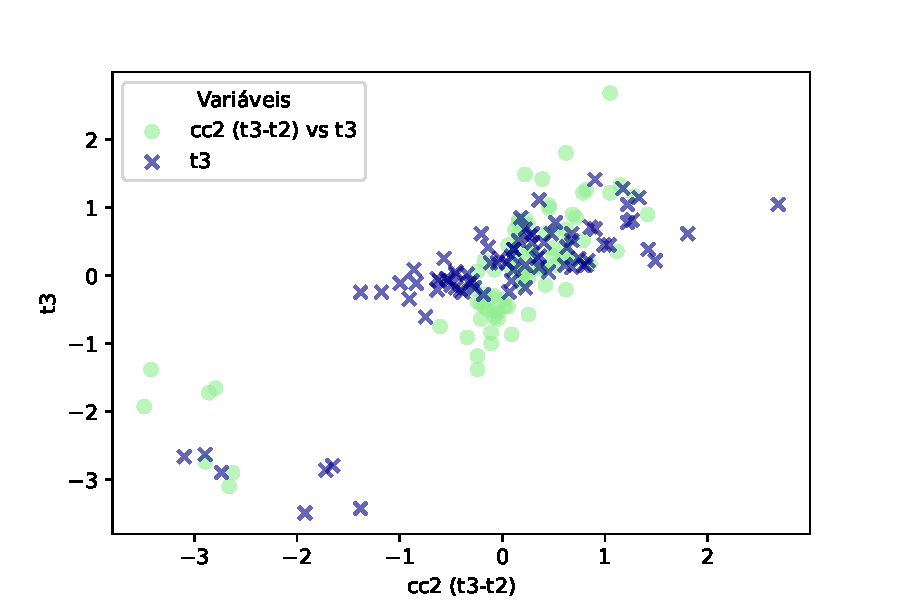
\includegraphics[scale=0.5]{figuras/Spearman/cc2-t3.pdf}
    \vspace{0.3cm} 
    % \caption{A alta correlação entre essas variáveis sugere que o tempo t3 tem uma influência considerável sobre o intervalo cc2, refletindo uma associação significativa no desenvolvimento embrionário. }
    \begin{minipage}{\linewidth}
        \centering
    \end{minipage}
\end{figure}
\FloatBarrier

A correlação entre \textit{cc2 e Ploidia (-0.03)} é muito fraca e negativa, sugerindo que não existe uma conexão relevante entre esses dois componentes. Isso indica que \textbf{o período temporal entre t3 e t2 não tem um impacto significativo na Ploidia}, o que sugere que o desenvolvimento temporal do embrião, simbolizado por cc2, não está diretamente ligado à ploidia do embrião.

\subsection*{cc3 (t5-t3)}
A correlação com \textit{t2 (0.15)} é fraca e positiva. Com \textit{t3 (0.25)}, a correlação é moderada e positiva, mostrando um ligeiro crescimento em cc3 à medida que t3 se eleva. A correlação com \textit{t4 (0.26)} é igualmente moderada e positiva. A correlação com \textit{t5 (0.81)} é extremamente forte e positiva, sugerindo que \textbf{conforme t5 cresce, cc3 também cresce quase de maneira linear}. Isso é coerente, já que cc3 é determinado como a diferença entre t5 e t3, e qualquer alteração em t5 afeta diretamente cc3. Por fim, a correlação com o \textbf{t8 (0.40)} é moderada e positiva, indicando que, conforme o t8 se eleva, o cc3 tende a crescer.

A correlação entre o intervalo \textit{t5-t3 (representado por cc3)} e o intervalo \textit{t5-t2 (0.90)} é extremamente forte e positiva, \textbf{sugerindo que o comportamento de cc3 está fortemente ligado ao intervalo t5-t2}. Portanto, o intervalo t5-t2 pode ser um indicador relevante para prever o comportamento de cc3, indicando que \textbf{a evolução do embrião entre os estágios t5 e t2 desempenha um papel relevante no comportamento de cc3 (t5-t3)}. Isso indica que alterações nesse intervalo temporal afetam significativamente a diferença de tempo entre os estágios t5 e t3. 

A correlação de cc3 com a \textit{Ploidia (-0.281)} é bastante elevada quando comparada a outras variáveis, como a correlação de Ploidia com t2 (-0.075) ou t5 (-0.237). Isso sugere que \textbf{cc3 exerce uma influência moderada e negativa sobre a Ploidia, indicando que alterações na cc3 podem ter um impacto relevante sobre a ploidia}. Este efeito adverso indica que alterações em cc3 estão ligadas a uma diminuição no valor da ploidia.

\subsection*{t5-t2}
A correlação com \textit{Morfo (-0.38)} é moderadamente negativa, sugerindo que, conforme o valor de Morfo cresce, o intervalo t5-t2 tende a se estreitar. Isso indica que \textbf{as características morfológicas do embrião podem influenciar o comportamento temporal entre os estágios t5 e t2}, possivelmente indicando um desenvolvimento mais devagar ou desordenado conforme as características morfológicas se modificam.

Com \textit{t3 (0.51)}, a correlação é moderada e positiva, sugerindo uma correlação mais intensa entre os intervalos temporais dos estágios t5 e t3. A correlação com \textit{t4 (0.39)} também é moderada e positiva. Com \textit{t5 (0.92)}, a correlação é extremamente intensa e positiva, sinalizando que \textbf{o período entre t5 e t2 está fortemente ligado ao tempo de t5. Isso é esperado, pois t5 representa o término desse intervalo}. A correlação robusta indica que \textbf{alterações em t5 afetam consideravelmente o intervalo entre t5 e t2}. A correlação com \textit{t8 (0.45)} é positiva e moderada, indicando uma conexão entre t8 e o intervalo t5-t2.

Com \textit{tSB (0.40) e tB (0.37)}, as correlações são moderadas e positivas, indicando que \textbf{a mudança nos tempos tSB e tB também afeta o intervalo entre t5 e t2}. No caso de \textit{s3 (indicado por t8-t5, -0.41)}, a correlação é moderada e negativa, indicando que, \textbf{conforme o intervalo t8-t5 cresce, o intervalo t5-t2 tende a se reduzir, indicando um possível comportamento compensatório entre os dois períodos de tempo}.

O coeficiente de correlação de \textbf{Ploidia (-0.23)} com t5-t2 é moderado e negativo, sugerindo \textbf{uma relação inversa entre as alterações na ploidia e o intervalo entre t5 e t2}. Isso indica que, \textbf{conforme t5-t2 evolui, a ploidia tende a se reduzir, indicando uma possível restrição da ploidia no comportamento temporal entre esses estágios}. 

\subsection*{s2 (t4-t3)}
A correlação com \textit{t3 (-0.22)} é moderada e negativa, sugerindo que conforme o valor de t3 cresce, a distância s2 (t4-t3) tende a se afilar. Isso indica que uma alteração no tempo t3 pode diminuir a distância entre t4 e t3, sugerindo que as alterações no tempo t3 estão um pouco inversamente ligadas a esse intervalo.

A correlação com \textit{cc2 (t3-t2) (-0.21)} é moderada e negativa. Isso pode sugerir uma relação inversa entre o comportamento temporal dos intervalos t4-t3 e t3-t2, com alterações em cc2 impactando negativamente o intervalo s2, possivelmente por causa de um comportamento mais rápido no começo do desenvolvimento do embrião.

Com uma correlação moderada e positiva de \textit{s3 (t8-t5) (0.25)}, indica que um crescimento no intervalo s3 está ligado a um crescimento no intervalo s2. Isso pode sugerir que \textbf{o aumento do intervalo entre t8 e t5 está ligado ao aumento do intervalo entre t4 e t3}, o que pode representar uma compensação nos tempos entre as diversas fases do embrião.

A correlação com \textit{Ploidia (0.11)} é leve e positiva, sugerindo que alterações em s2 exercem um efeito levemente positivo na ploidia. Apesar do efeito ser mínimo, ele propõe que \textbf{uma alteração em s2 pode levar a uma pequena alteração na ploidia}.

\subsection*{s3 (t8-t5)}
A correlação com \textit{t5 (-0.39)} é moderada e negativa. Isso indica que \textbf{o período entre t8 e t5 diminui à medida que o estágio t5 progride, sugerindo que uma elevação em t5 pode levar a uma aceleração do progresso}, reduzindo o intervalo subsequente até t8. 

Com \textit{t8 (0.48)}, a correlação é positiva e moderada mais alta que t5, indicando que, conforme t8 se eleva, o intervalo s3 também tende a se expandir. Isso sugere que um aumento no intervalo de tempo entre t8 e t5 está ligado a um incremento no valor de t8, sinalizando um processo de evolução mais extenso ou mais lento em comparação com outros intervalos. \textbf{Este resultado indica que, conforme o embrião se aproxima do estágio t8, o período de tempo entre os estágios t8 e t5 aumenta}, assim demonstrado no gráfico abaixo, em que s3 está em ver claro. 

\begin{figure}[h]
    \captionsetup{font=footnotesize, justification=centering, labelsep=period, position=above}
    \caption{Dispersão entre s3 (t8-t5) e t8 - Coeficiente de Spearman: 0.48}
    \label{fig:s3-t8}
    \centering
    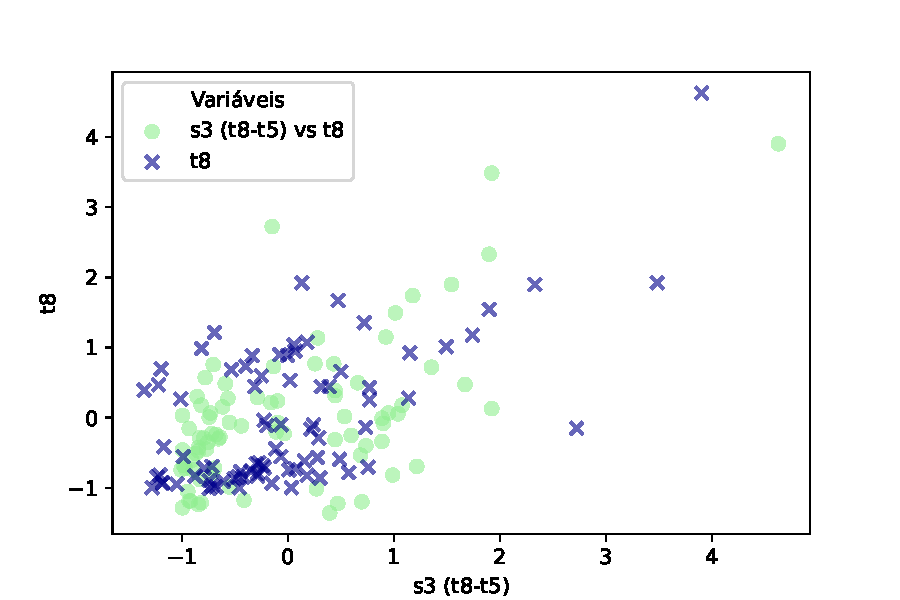
\includegraphics[scale=0.4]{figuras/Spearman/s3-t8.pdf}
    \vspace{0.3cm} 
    % \caption{A correlação moderada entre essas duas variáveis indica que há uma associação entre elas, embora outros fatores possam estar influenciando essa relação.}
    \begin{minipage}{\linewidth}
        \centering
    \end{minipage}
\end{figure}
\FloatBarrier

A correlação com \textit{cc3 (t5-t3) (-0.36)} é moderada e negativa. Este efeito indica que uma extensão prolongada entre t5 e t3 pode estar ligada a uma diminuição no tempo entre t8 e t5.

Finalmente, a correlação com a \textit{Ploidia (0.25)} é moderada e positiva, indicando que, conforme a ploidia cresce, o intervalo s3 (t8-t5) também tende a se expandir. Este efeito pode sugerir que a \textbf{aneuploidia está ligado a uma diminuição no tempo de desenvolvimento, estendendo o intervalo entre t8 e t5}.

\subsection*{tSC-t8}
A relação com \textit{t8 (-0.29)} é moderadamente negativa sugere que, conforme o intervalo de tempo entre tSC e t8 cresce, o tempo de t8 também tende a crescer. Este resultado indica que,\textbf{ ao aumentar o intervalo entre tSC e t8, pode ocorrer uma diminuição na velocidade do desenvolvimento embrionário entre tSC e t8, estendendo o período até t8}. Isso pode indicar uma etapa de crescimento mais lenta ou prolongada, influenciando o ritmo geral de avanço do embrião.

A correlação com \textit{tSC (0.70)} é forte e positiva, que indica que o intervalo tSC-t8 tem uma ligação direta com o intervalo tSC. \textbf{Conforme o intervalo de tempo entre tSC e t8 se amplia, o intervalo tSC também tende a se expandir}. \textbf{Este efeito indica uma relação temporal na qual o estágio tSC desempenha um papel significativo no progresso do embrião no período subsequente até t8}.

A correlação de \textit{tB-tSB (0.20)} é positiva e indica que um crescimento no intervalo entre tB e tSB pode estar estreitamente ligado a um crescimento no intervalo tSC-t8. 

A correlação muito tênue \textit{(0.04)} e positiva sugere que Ploidia exerce uma influência quase nula no intervalo tSC-t8. 

\subsection*{tB-tSB}
A correlação com a \textit{Idade (0.20)} sendo positiva e fraca indica que, conforme a idade avança, o intervalo tB-tSB também tende a crescer, mesmo que de maneira sutil. Isso pode sugerir que a idade da paciente pode ter um pequeno impacto no desenvolvimento embrionário, possivelmente indicando uma variação no ritmo de desenvolvimento.

A correlação moderadamente positiva do \textit{Estágio (0.38)} indica que, conforme o estágio de desenvolvimento progride, o intervalo tB-tSB tende a se estender. 

A correlação moderadamente positiva de \textit{tB (0.38)} indica que, conforme o intervalo tB se amplia, o intervalo tB-tSB também tende a se expandir. Isso é coerente, já que \textbf{o período tB é um estágio inicial do desenvolvimento embrionário, e sua duração pode impactar diretamente o tempo até o estágio seguinte}, o tSB, impactando a evolução do desenvolvimento embrionário. Uma maior extensão do tB geralmente indica um período mais extenso até o tSB.

A correlação com \textit{Ploidia (-0.284)} exerce um efeito significativo, visto que \textbf{é a segunda correlação de maior magnitude entre as variáveis examinadas}. Desempenha um papel significativo, uma vez que indica que a qualidade genética do embrião, avaliada por tB e tSB, pode impactar diretamente a ploidia. 

\subsection*{Ploidia}
A avaliação das variáveis relacionadas à ploidia indica que \textbf{a idade materna tem o maior efeito na qualidade genética do embrião}. A idade materna, \textbf{com uma correlação de -0,50}, apresenta uma correlação inversa significativa com a ploidia. Isso significa que, \textbf{conforme a mulher envelhece, a quantidade de embriões euploides diminui, o que indica um crescimento na taxa de aneuploidia}. Isso está alinhado com o que a literatura já aponta sobre o impacto do envelhecimento materno na qualidade genética dos embriões, onde embriões de mulheres mais idosas têm maior probabilidade de conter erros cromossômicos. 

Adicionalmente, as variáveis \textbf{tB-tSB e cc3 (t5-t3)} possuem uma correlação moderada de -0,28 com a ploidia, sugerindo que o período entre as fases de desenvolvimento \textbf{t5, t3, tB e tSB podem afetar diretamente a qualidade genética do embrião}. Este intervalo de tempo está ligado ao ritmo de divisão celular e ao comportamento dos cromossomos. Mudanças nesse processo podem comprometer a criação de embriões euploides, levando a um aumento na probabilidade de aneuploidia. 

Outros fatores, como o \textbf{estágio de desenvolvimento (-0,24) e o t5 (-0,24)}, também mostraram uma correlação negativa com a ploidia. Isso indica que \textbf{o avanço para fases mais avançadas de desenvolvimento e o atraso no t5 podem estar ligados a uma queda na qualidade genética dos embriões}. 

\subsubsection{Atividade 4 (A4): Separar o conjunto de dados em conjuntos de treinamento, validação e teste, fazendo uma distribuição dos dados e aplicar técnica de aumento de dados}

\subsection*{Divisão do Conjunto de Dados em Treinamento e Validação}

Foi realizada a divisão do conjunto de dados normalizado em dois subconjuntos principais: \textbf{conjunto de treinamento} (80\%) e \textbf{conjunto de validação} (20\%). Essa segmentação foi feita com estratificação em relação à variável-alvo \texttt{Ploidia}, assegurando que a proporção entre embriões euploides e aneuploides fosse preservada em ambos os conjuntos.

A divisão foi implementada de forma aleatória, com o intuito de evitar viéses associados à ordenação dos dados. Essa aleatoriedade contribui para a geração de subconjuntos mais representativos e imparciais, como indicado por \citeonline{andrew2018}, e é particularmente relevante quando se trabalha com conjuntos de dados de pequeno porte.

\subsection*{Balanceamento das Classes no Conjunto de Treinamento}
Para evitar que o modelo aprenda de forma enviesada devido a desbalanceamentos entre as classes, foi implementada uma etapa de \textbf{balanceamento do conjunto de treinamento}. O procedimento consistiu na aplicação de uma técnica inspirada em \textit{under-sampling}: a classe majoritária foi reduzida até igualar-se à classe minoritária em número de amostras. No entanto, ao invés de descartar os dados excedentes, eles foram realocados para o conjunto de validação. Isso permitiu manter o conjunto de treinamento equilibrado sem perder as informações contidas nas instâncias adicionais.

Essa abordagem mitigou os riscos de sobreajuste (overfitting) para a classe dominante e fortaleceu a avaliação do modelo com um conjunto de validação mais representativo. Conforme discutido por \citeonline{ercemapi}, esse tipo de técnica é especialmente útil em contextos biomédicos, onde o volume de dados pode ser restrito e a preservação da representatividade é essencial para garantir confiabilidade. 

\subsection*{Aumento de Dados (\textit{Data Augmentation}) utilizando o Método de Monte Carlo} 
Para aumentar a capacidade de generalização do modelo e reduzir o risco de \textit{overfitting}, foi aplicada uma técnica de \textbf{aumento de dados} (\textit{data augmentation}) baseada em amostragem estocástica — uma variação do método de Monte Carlo.

Este processo gerou novas amostras sintéticas com base nas propriedades estatísticas das variáveis numéricas do conjunto original. A geração seguiu os seguintes critérios:
\begin{itemize}
    \item Para \textbf{variáveis numéricas}, os novos valores foram gerados a partir de uma distribuição normal, usando como parâmetros a média e o desvio padrão da variável original.
    \item Para \textbf{variáveis categóricas}, os valores foram replicados aleatoriamente com reposição, de forma proporcional à sua distribuição original.
\end{itemize}

A aplicação da média e do desvio padrão assegura que os novos dados numéricos correspondam às características do conjunto original, ao mesmo tempo que as categorias mantêm suas proporções, mantendo os padrões originais. A produção de dados por meio de distribuições estatísticas amplia a diversidade do conjunto sem adicionar ruído excessivo ou padrões inverossímeis, assegurando uma diversificação controlada. Este procedimento garante que o conjunto de treinamento ampliado seja robusto o suficiente para treinar o modelo, prevenindo sobrecargas e aprimorando a generalização, levando a um modelo mais eficiente e seguro.

Depois de executar o código, a base de dados de treinamento foi  \textbf{ampliada em 20 vezes}, conforme o fator de aumento definido. As amostras sintéticas geradas foram concatenadas ao conjunto original, totalizando um volume significativamente maior de dados. Essa abordagem é especialmente indicada em contextos onde o conjunto de dados é escasso, como em estudos biomédicos, e contribui para a construção de modelos mais estáveis, com maior capacidade de reconhecer padrões complexos e realizar previsões confiáveis em novos dados.

\section{Fase 2: Desenvolvimento e Avaliação do Modelo}
\subsection{OE2 - Treinar e Ajustar do Modelo de Machine Learning para Predição de Euploidia}
\subsubsection{Atividade 5 (A5): Desenvolvimento e Treinamento do Modelo de Machine Learning para Otimização da Predição de Euploidia}
Nesta etapa do projeto, foi desenvolvido e treinado um modelo de Aprendizado de Máquina (Machine Learning) com o objetivo de otimizar a predição de ploidia em embriões, utilizando dados morfocinéticos extraídos do Time-Lapse System (TLS). O modelo escolhido foi uma Rede Neural Artificial do tipo Perceptron Multicamadas (MLP, do inglês Multilayer Perceptron), implementada com a biblioteca Scikit-Learn em linguagem Python.

A \textbf{Scikit-Learn} foi empregada para \textit{diversas tarefas essenciais do pipeline de modelagem}, incluindo: a divisão dos dados em conjuntos de treino e teste com estratificação, a padronização dos atributos com \texttt{StandardScaler}, o treinamento da rede neural com \texttt{MLPClassifier} e a avaliação do modelo por meio de métricas como acurácia, curva ROC e matriz de confusão. Além disso, a Scikit-Learn também foi responsável pela serialização do modelo e do scaler com a ferramenta \texttt{joblib}, permitindo seu reaproveitamento em outras etapas do sistema. Essa integração modular e coesa entre diferentes etapas do processo de modelagem é um dos principais pontos fortes da Scikit-Learn, se tornando particularmente adequada para projetos como esse, que exigem reprodutibilidade, clareza na implementação e robustez computacional \cite{geron2017}.

A arquitetura de Rede Neural Artificial utilizada foi o \textbf{Perceptron Multicamadas} (MLP, do inglês \textit{Multilayer Perceptron}), que é uma rede supervisionada composta por três tipos de camadas: uma de entrada, uma ou mais ocultas e uma de saída \cite{haykin2009}. O modelo MLP foi construído utilizando a classe \texttt{MLPClassifier}, da biblioteca Scikit-Learn, que é um algoritmo de aprendizado supervisionado baseado em Redes Neurais Artificiais que utiliza o algoritmo de retropropagação do erro para realizar a otimização dos pesos durante o treinamento \cite{geron2017}.  Essa classe faz parte do módulo \texttt{sklearn.neural\_network} e oferece uma interface padronizada para treinamento e predição, integrando facilmente ao restante do ecossistema da Scikit-Learn, como ferramentas de validação cruzada, seleção de atributos e ajuste de hiperparâmetros \cite{geron2017}. 

A configuração do modelo incluiu os seguintes hiperparâmetros principais:
\begin{itemize}
  \item \textbf{activation='relu'}: Utiliza a função de ativação ReLU (Rectified Linear Unit), pra evitar o problema do desvanecimento do gradiente \cite{geron2017}.
  \item \textbf{solver='adam'}: Aplica o otimizador \textit{Adam}, um método de descida do gradiente adaptativo eficiente para volumes de dados e parâmetros.
  \item \textbf{max\_iter=1000}: d o número máximo de iterações para o treinamento, garantindo convergência adequada.
  \item \textbf{random\_state=attempt}: Usado para reprodutibilidade dos resultados.
\end{itemize}

Após o treinamento, os objetos do modelo e do \textit{scaler} foram serializados em arquivos \texttt{.pkl} utilizando a ferramenta \texttt{joblib}. O \textbf{scaler} é um objeto responsável pela normalização dos dados, neste caso, utilizando a padronização por Z-Score \cite{geron2017}, garantindo que todas as variáveis contribuam de forma equilibrada para o aprendizado. É fundamental aplicar exatamente a mesma transformação aos dados futuros que serão analisados pelo modelo, razão pela qual o objeto do \textit{scaler} é salvo junto ao modelo treinado. Já o arquivo com extensão \texttt{.pkl} (do inglês \textit{Pickle}) é utilizados para armazenar os objetos Python de forma persistente no disco. A serialização dos objetos, modelo treinado e scaler, permite que eles sejam carregados posteriormente sem a necessidade de repetir todo o processo de treinamento, otimizando tempo, desempenho e consistência da aplicação.

Foi incorporado ao pipeline do projeto o método \textit{LIME} (Local Interpretable Model-Agnostic Explanations). O LIME é uma técnica de Inteligência Artificial Explicável (XAI — \textit{Explainable Artificial Intelligence}) proposta por \citeonline{ribeiro2016}, que visa interpretar modelos complexos de forma local e intuitiva. Sua principal função é explicar individualmente cada predição feita por modelos considerados “caixas-pretas”, como redes neurais. O LIME faz isso criando um modelo interpretable treinado em uma vizinhança gerada artificialmente em torno da instância original de entrada. Assim, ele estima quais atributos (características) mais influenciaram a decisão do modelo naquela predição específica \cite{ribeiro2016}. 

Para tornar as predições do modelo mais compreensíveis para embriologistas e profissionais da área clínica, foi utilizada a ferramenta LIME (Local Interpretable Model-Agnostic Explanations), uma técnica de Inteligência Artificial Explicável (XAI) proposta por \citeonline{ribeiro2016}. Essa técnica permite interpretar individualmente cada predição feita pela rede neural, identificando quais atributos mais contribuíram para a classificação de cada embrião como euploide ou aneuploide. No presente projeto, a porcentagem de euploidia de cada embrião foi estimada com base na probabilidade de predição da classe "euploide" (classe 1) fornecida pelo modelo MLP, por meio do método \texttt{predict\_proba()}. Esse valor probabilístico foi convertido em percentual  na planilha final gerada pelo sistema. Esse tipo de abordagem interpretável é especialmente importante em contextos biomédicos, onde decisões automatizadas exigem justificativas claras e auditáveis \cite{arrieta2020, ribeiro2016}.

Ao aplicar o modelo preditivo em novos dados, a entrada inicial, uma planilha contendo os dados morfocinéticas dos embriões, passa por um processo de pré-processamento automatizado. Esse pipeline transforma variáveis originalmente categóricas, como classificações textuais da morfologia embrionária, em valores numéricos padronizados. Um exemplo dessa transformação é a classificação morfológica, que é convertida automaticamente em categorias numéricas que representam níveis de qualidade embrionária, conforme descrito na metodologia. Após essa etapa, os dados numéricos são submetidos a um escalonamento por meio de um \textit{scaler}, que normaliza as variáveis para uma mesma escala, evitando que diferenças de magnitude influenciem indevidamente a predição. Em seguida, o modelo de Rede Neural MLP realiza a predição da classe para cada embrião, classificando-os como euploides ou aneuploides. Assim, o modelo fornece a probabilidade associada à predição da classe euploide, expressa em termos percentuais. Finalmente, os resultados (que incluem as informações originais da planilha, a classificação prevista e a probabilidade de euploidia) são exportados para um novo arquivo. Essa saída organizada facilita a interpretação dos dados e suporta a tomada de decisão clínica, tornando o processo mais transparente e acessível.

\subsection{OE3 - Realizar Avaliação do Modelo}
\subsubsection{Atividade 6 (A6): Utilizar métricas adequadas para medir o desempenho do modelo}
Nesta etapa, foram aplicadas métricas quantitativas para avaliar o desempenho do modelo de aprendizado de máquina desenvolvido para a predição de euploidia em embriões. A \textbf{acurácia} de 88,2\% indica que o modelo classificou corretamente a grande maioria dos embriões, tanto euploides quanto aneuploides, mostrando uma performance geral satisfatória. A \textbf{Área sob a Curva ROC (AUC)} de 0,944 evidencia a elevada capacidade do modelo em distinguir entre as classes, mesmo ao variar o limiar de decisão. 

O \textbf{recall}, que mensura a taxa de verdadeiros positivos, apresentou resultados diferenciados para as classes: foi perfeito para embriões aneuploides (1,00), garantindo a identificação correta de todos os casos com anomalias genéticas, e robusto para embriões euploides (0,75), indicando uma boa sensibilidade, ainda que com espaço para melhorias. Esses indicadores superaram os critérios mínimos estabelecidos para aceitação do modelo.

A matriz de confusão gerada (Figura~\ref{fig:matrizDeConfusao}) revela que, dentre os 17 embriões avaliados na base de teste, 9 embriões aneuploides foram corretamente classificados (verdadeiros negativos) e 6 euploides foram corretamente identificados (verdadeiros positivos). Apenas dois casos de euploidia foram incorretamente classificados como aneuploides (falsos negativos) e nenhum aneuploide foi erroneamente identificado como euploide (falso positivo).

\begin{figure}[h]
    \captionsetup{font=footnotesize, justification=centering, labelsep=period, position=above}
    \caption{Matriz de confusão para avaliação do desempenho do modelo}
    \label{fig:cmatrizDeConfusao}
    \centering
    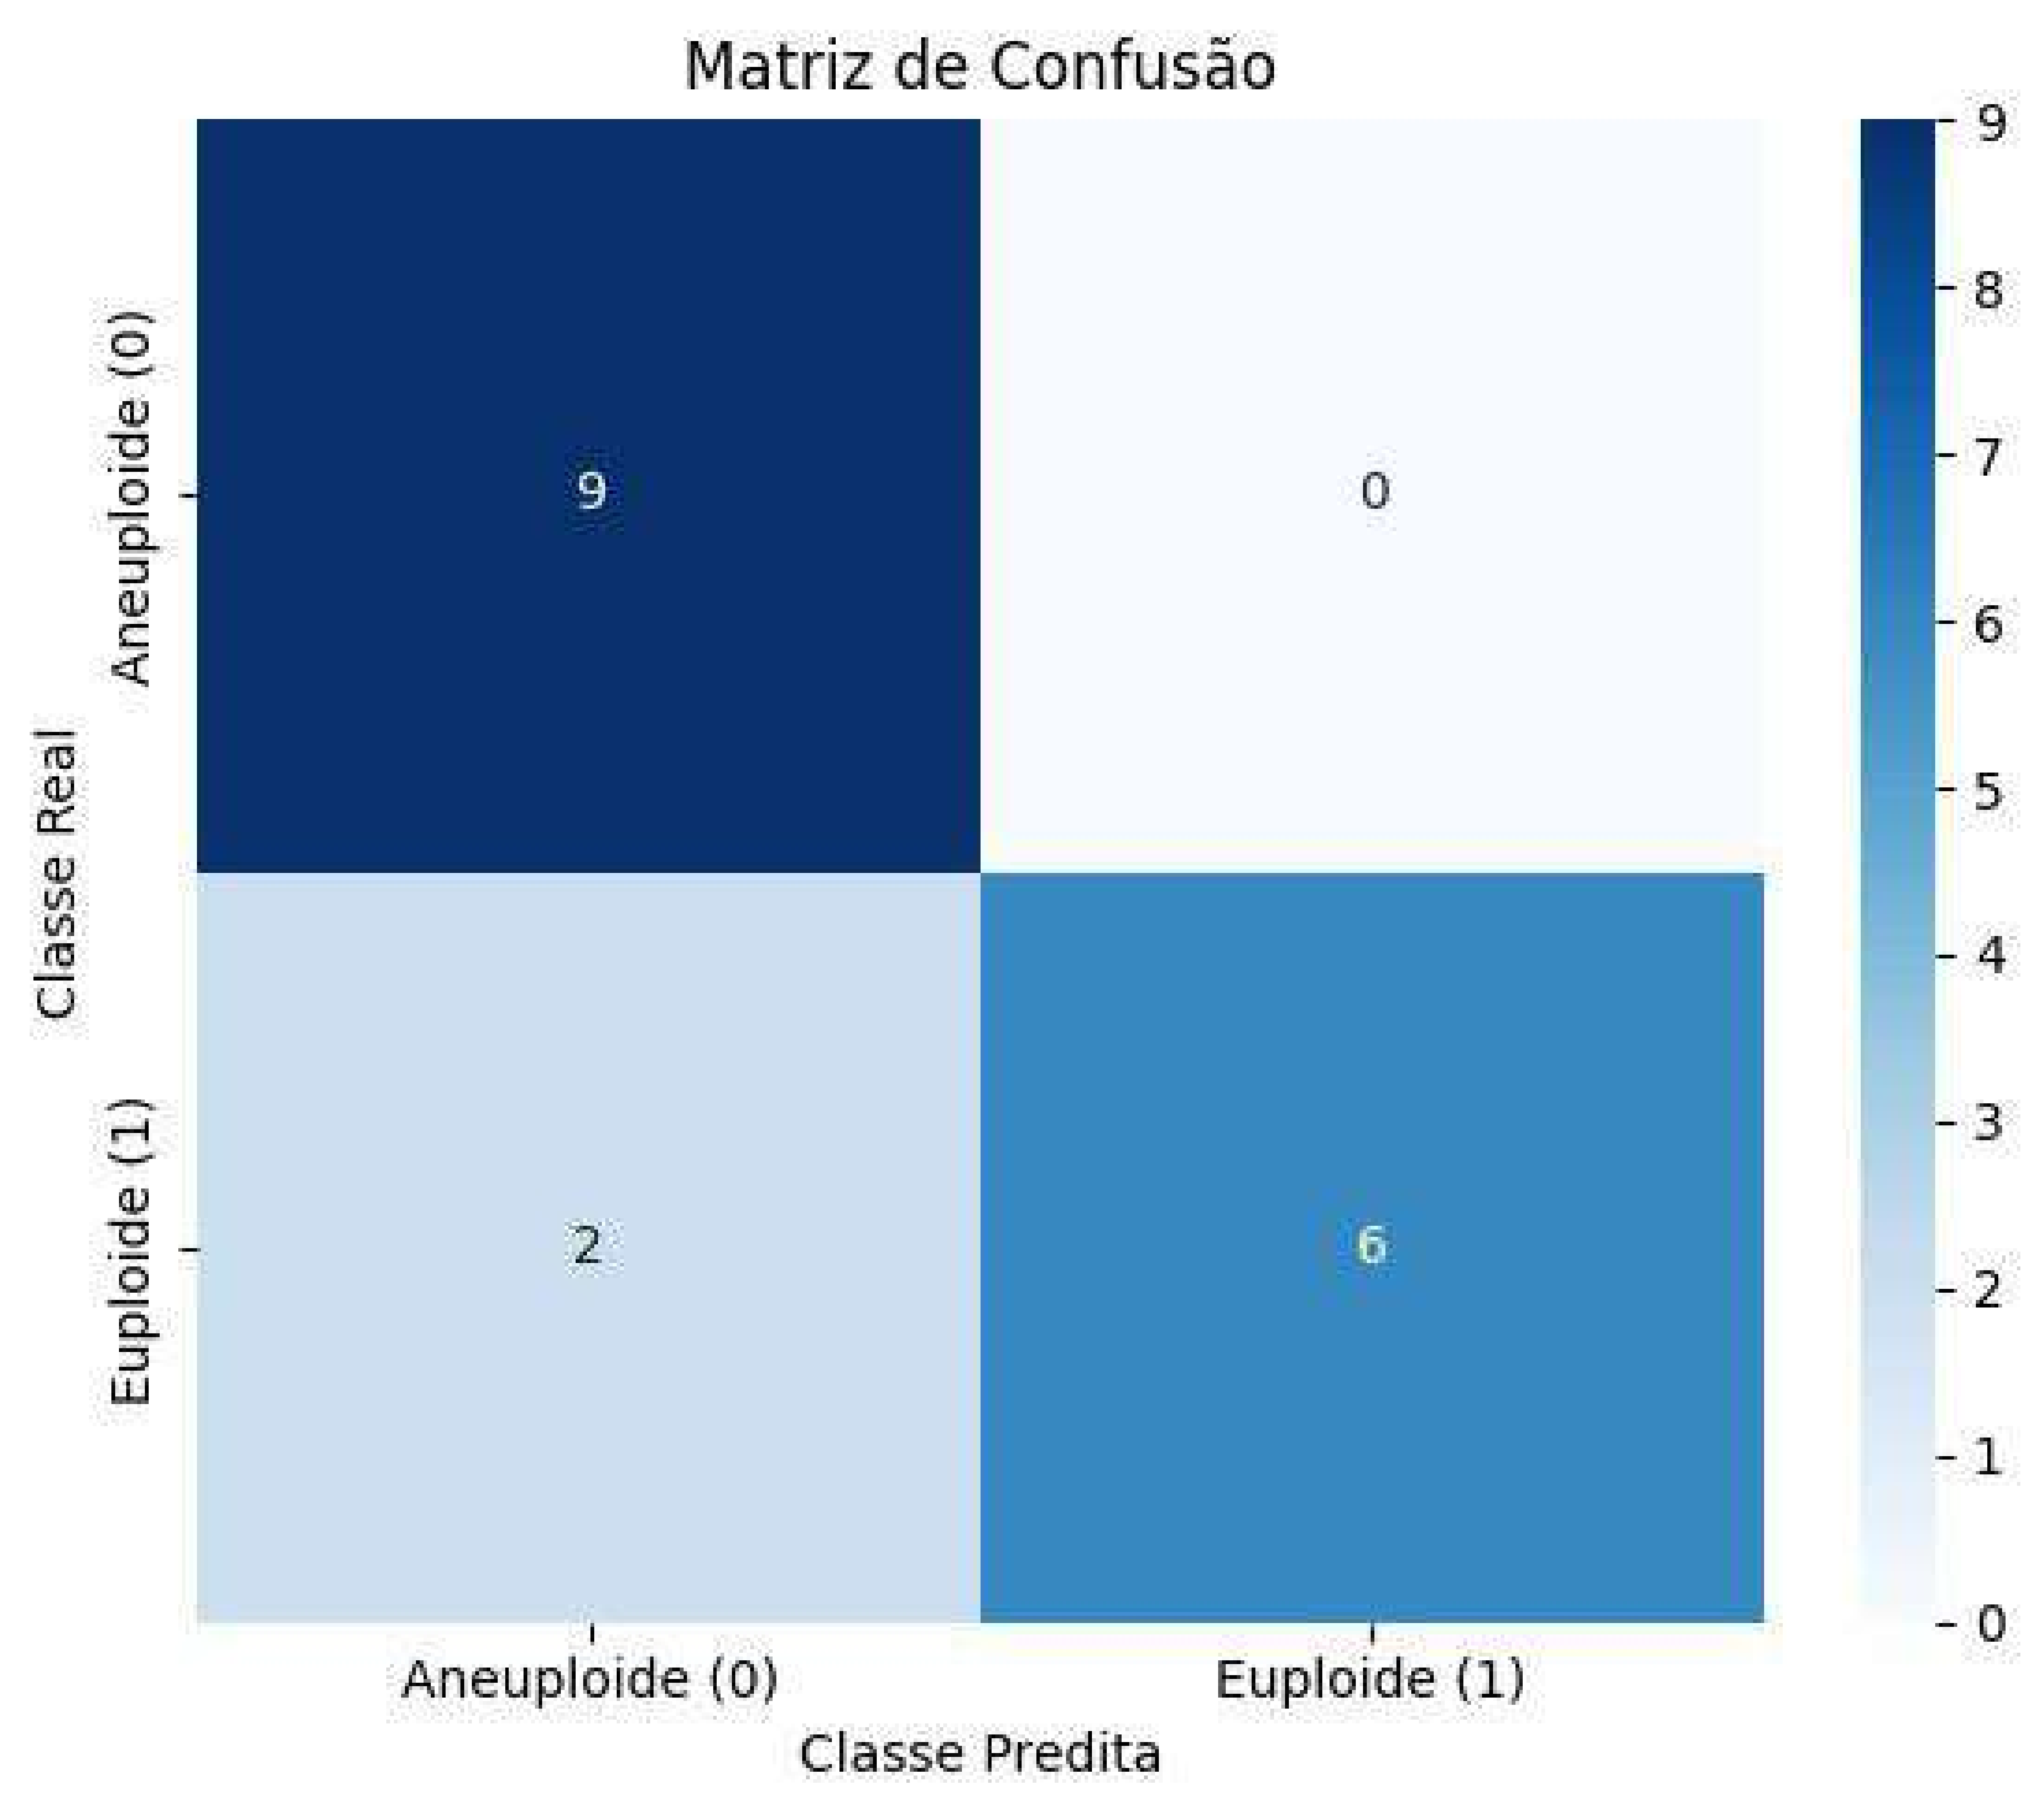
\includegraphics[scale=0.11]{figuras/IA/matrizDeConfusao.pdf}
\end{figure}
\FloatBarrier

A curva ROC (Receiver Operating Characteristic), ilustrada na Figura~\ref{fig:curvaRoc}, expressa graficamente a performance do classificador sob diferentes limiares de decisão. A área sob a curva ROC (AUC) foi de 0,94, o que indica excelente capacidade do modelo em distinguir entre as duas classes.

\begin{figure}[h]
    \captionsetup{font=footnotesize, justification=centering, labelsep=period, position=above}
    \caption{Curva ROC com AUC de 0,94.}
    \label{fig:curvaRoc}
    \centering
    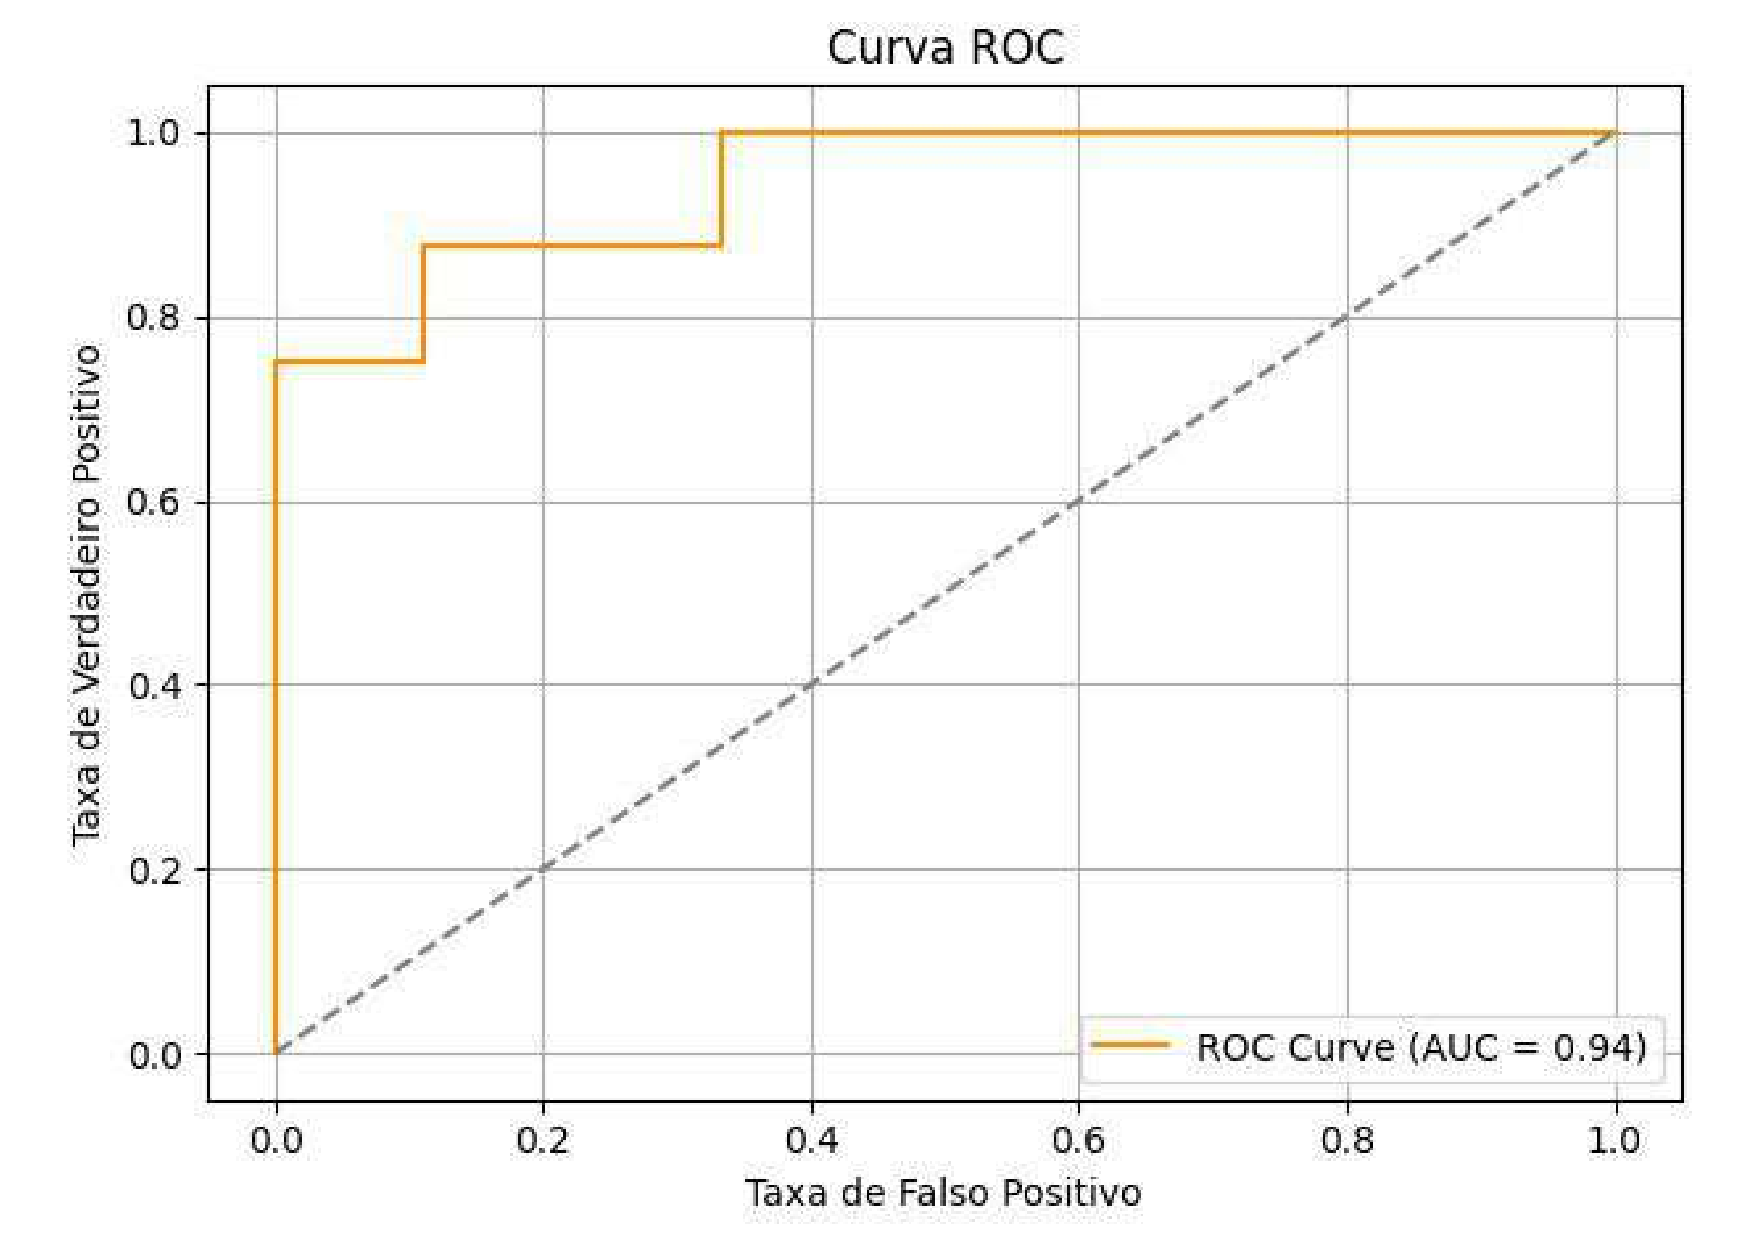
\includegraphics[scale=0.4]{figuras/IA/curvaRoc.pdf}
\end{figure}
\FloatBarrier

Com base nas métricas obtidas e nas representações gráficas, se conclui que o modelo treinado apresentou desempenho consistente. A elevada acurácia e AUC, aliadas ao recall para embriões aneuploides, reforçam a confiabilidade do modelo como uma ferramenta auxiliar na triagem embrionária. Esses resultados evidenciam a viabilidade de aplicar técnicas de aprendizado de máquina, como redes neurais, no suporte à tomada de decisão em contextos de reprodução assistida.

\subsubsection{Atividade 7 (A7): Avaliação do Desempenho do Modelo na Predição por Meio da Matriz de Confusão e Curva ROC}
A \textbf{matriz de confusão} explicada na Atividade 6 (A6) é uma representação tabular que resume o desempenho do classificador ao comparar os rótulos reais com as previsões do modelo. Ela permite a identificação de quatro métricas essenciais:

\begin{itemize}
    \item \textbf{Verdadeiros Positivos (TP)}: Casos em que o modelo previu corretamente a euploidia (classe 1). Foram identificados 6 TP.
    \item \textbf{Verdadeiros Negativos (TN)}: Casos em que o modelo previu corretamente a aneuploidia (classe 0). Foram registrados 9 TN.
    \item \textbf{Falsos Positivos (FP)}: Casos em que o modelo previu incorretamente um embrião aneuploide como euploide. Neste caso, FP = 0.
    \item \textbf{Falsos Negativos (FN)}: Casos em que o modelo classificou incorretamente um embrião euploide como aneuploide. Foram observados 2 FN.
\end{itemize}

Essas métricas permitem calcular indicadores importantes, como \textbf{precisão}, \textbf{recall}, \textbf{especificidade} e \textbf{acurácia}. A matriz resultante confirma o excelente desempenho do modelo na detecção de aneuploidias, com zero falsos positivos e todos os embriões com anomalias genéticas corretamente identificados.

O gráfico da Figura~\ref{fig:sensibilidade} apresenta a variação das métricas de \textbf{sensibilidade} e \textbf{especificidade} do modelo conforme diferentes valores de limiar de decisão, indo de 0 a 1. A \textbf{sensibilidade} (também chamada de recall para a classe euploide) representa a proporção de embriões euploides corretamente identificados como tais. Observa-se que ela decresce à medida que o limiar aumenta, indicando que o modelo se torna mais conservador na predição de euploidia,o que reduz a quantidade de verdadeiros positivos (euploides corretamente classificados). Por outro lado, a \textbf{especificidade} (ou recall para a classe aneuploide) tende a aumentar com o aumento do limiar, o que significa que o modelo passa a cometer menos falsos positivos, classificando embriões aneuploides de forma mais precisa como negativos. Esse gráfico revela o clássico \textit{trade-off} entre sensibilidade e especificidade. Ao escolher limiares mais baixos, há maior sensibilidade (maior detecção de euploidia), mas menor especificidade (mais risco de falsos positivos). Já limiares mais altos priorizam a especificidade, reduzindo a chance de classificar incorretamente um aneuploide como euploide, mas podem deixar de identificar euploidias verdadeiras. Essa análise é essencial para aplicações clínicas, nas quais a escolha do limiar pode ser ajustada com base em prioridades médicas, como evitar falsos negativos (não detectar um embrião viável) ou falsos positivos (implantar um embrião inviável).

\begin{figure}[h]
    \captionsetup{font=footnotesize, justification=centering, labelsep=period, position=above}
    \caption{Relação entre sensibilidade e especificidade em diferentes limiares de decisão.}
    \label{fig:sensibilidade}
    \centering
    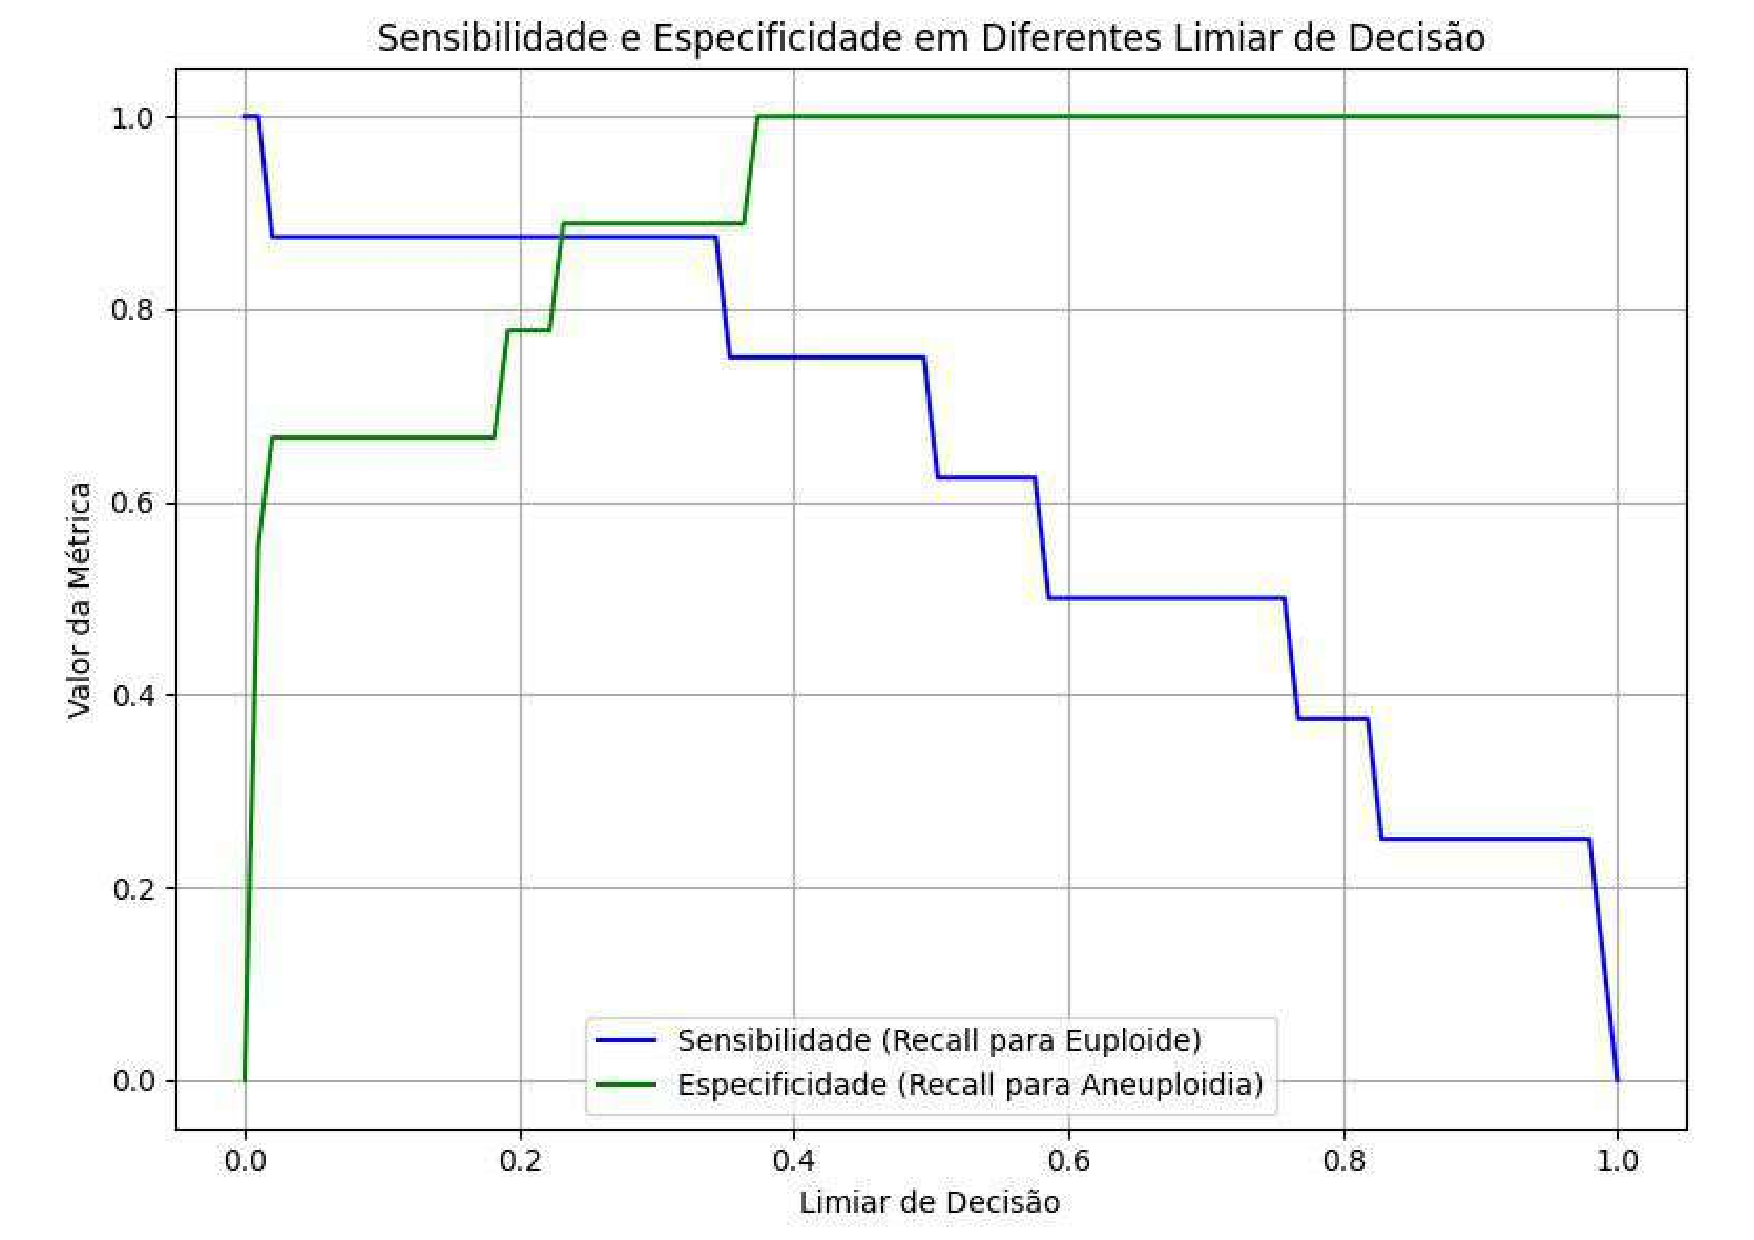
\includegraphics[scale=0.45]{figuras/IA/sensibilidade.pdf}
\end{figure}
\FloatBarrier

Dessa forma, a análise da matriz de confusão e da curva de sensibilidade versus especificidade confirma que o modelo apresenta excelente desempenho, especialmente na identificação de embriões aneuploides. A ausência de falsos positivos e a possibilidade de ajustar o limiar de decisão conforme a prioridade clínica tornam o modelo uma ferramenta promissora.

\subsection{OE4 - Construir Protótipo}
\subsubsection{Atividade 8 (A8): Prototipar uma interface básica para exibir as predições de euploidia para o usuário final (médicos)}
A execução da Atividade 08 teve início com a análise das necessidades essenciais para a construção de uma interface funcional, clara e objetiva voltada aos profissionais da área médica. O principal objetivo nesta etapa foi desenvolver um protótipo viável de interface — um \textit{Mínimo Produto Viável} (MVP) — que possibilitasse a visualização das predições de euploidia de maneira intuitiva, prática e segura. Como a intenção é evoluir progressivamente esse sistema, priorizou-se uma entrega enxuta, mas funcional, capaz de ser testada e aprimorada com base no feedback dos usuários finais.

A prototipação foi realizada utilizando a ferramenta \textbf{Figma}, que permitiu o desenvolvimento visual colaborativo e iterativo da solução. O MVP da interface consiste em uma estrutura simples com foco total na funcionalidade central: permitir que o usuário realize o \textit{upload} de uma planilha com dados morfocinéticos dos embriões e receba como resultado a predição da ploidia de cada um deles, incluindo a probabilidade estimada de euploidia.

O processo de construção da interface considerou os seguintes elementos:
\begin{itemize}
    \item \textbf{Header e Identidade do Projeto:} A interface possui um cabeçalho simples, com a identidade visual do projeto e um título claro que indica a finalidade da página.

    \item \textbf{Apresentação do Projeto:} Logo abaixo do cabeçalho, é exibido um resumo introdutório do projeto, explicando de forma objetiva a proposta da solução e sua relevância no contexto da medicina reprodutiva.

    \item \textbf{Equipe Envolvida:} A seção seguinte apresenta os participantes do projeto, incluindo o professor orientador, as alunas desenvolvedoras e o médico especialista em medicina reprodutiva

    \item \textbf{Restrições e Regras para o Upload:} Uma seção dedicada às instruções detalhadas orienta o usuário sobre os requisitos da planilha a ser submetida. São explicadas as colunas numéricas obrigatórias, seus nomes exatos e o formato esperado dos dados, com o intuito de evitar erros de entrada que comprometam a interpretação dos dados pelo modelo de inteligência artificial.

    \item \textbf{Upload e Validação de Arquivo:} A funcionalidade principal da interface é o envio da planilha. Foram integradas validações para evitar o envio incorreto de arquivos — etapa crítica para garantir a integridade dos dados analisados e a segurança da predição.

    \item \textbf{Página de Resultados:} Após o envio, o usuário é redirecionado a uma segunda página, que apresenta de forma clara os resultados da análise. São exibidos o total de embriões analisados, a quantidade classificada como euploide, a quantidade aneuploide e a probabilidade de euploidia associada a cada embrião.

\end{itemize}

A simplicidade do design foi uma escolha estratégica. Ao concentrar esforços no essencial, garantiu-se que o protótipo fosse funcional e acessível, respeitando as boas práticas de UX e as heurísticas de Nielsen já mencionadas. A proposta é que esse MVP sirva como base para iterações futuras, nas quais novas funcionalidades, como visualizações gráficas, histórico de análises ou exportação de relatórios, possam ser integradas com base nas necessidades dos médicos e especialistas que utilizarão o sistema.

A figura interativa do protótipo pode ser acessada por meio do link abaixo. Ela foi desenvolvida na plataforma Figma e representa a interface básica criada para visualização das predições de euploidia:

\begin{center}
    \href{https://www.figma.com/design/0AstYynXwZO9zVudP1NimJ/Predi%C3%A7%C3%A3o-de-Ploidia?node-id=1-2&t=GcDVvNcPFkmVPj8F-1}{\texttt{Preditor de Ploidia}}
\end{center}

Além disso, os \textit{frames} do Figma também estão disponíveis no repositório do projeto no GitHub, garantindo acesso futuro mesmo que o link original se torne indisponível.


\subsubsection{Atividade 9 (A9):  Desenvolver a aplicação web integrando o protótipo à inteligência artificial existente}
A implementação da solução web foi realizada com base nas tecnologias modernas descritas na metodologia: \textbf{Next.js com App Router}, \textbf{TypeScript}, \textbf{TailwindCSS}, e bibliotecas auxiliares para leitura de arquivos e comunicação com a API de predição. A execução teve início com a estruturação da aplicação através do comando \textit{create-next-app}, que gerou a base do projeto com suporte ao roteamento moderno e a organização de pastas voltada para escalabilidade.

Com a arquitetura inicial definida, a implementação do protótipo funcional foi iniciada com base no layout desenvolvido no Figma. A interface foi cuidadosamente construída para refletir o fluxo de uso planejado, garantindo uma transição fluida entre prototipagem e desenvolvimento. A cada componente implementado, houve o cuidado de seguir os princípios de \textbf{design centrado no usuário}, considerando clareza, legibilidade e acessibilidade, especialmente em um contexto sensível como o médico.

Durante o desenvolvimento, foram feitas diversas \textbf{validações e verificações} para assegurar a integridade dos dados. A aplicação possui mecanismos de checagem da planilha enviada pelo usuário, validando a presença e a estrutura correta das colunas esperadas, prevenindo erros durante o processamento e evitando que predições equivocadas sejam geradas por causa de entradas malformadas. Esse cuidado garante maior robustez à solução e confiança no uso clínico.

Para a \textbf{integração com o modelo de inteligência artificial}, foi utilizada a \textbf{FastAPI} como framework para a construção da API backend. A escolha da FastAPI se deu por sua performance elevada, suporte a tipagem com Pydantic, documentação automática via Swagger e facilidade de integração com aplicações front-end. Essa estrutura garantiu que a comunicação entre a interface e o modelo de IA ocorresse de forma fluida, eficiente e segura. Os dados enviados pela planilha são processados e retornam as predições com porcentagens de euploidia associadas a cada embrião, exibidas em tempo real para o usuário.

A aplicação foi \textbf{hospedada na plataforma Vercel}, que possibilitou um processo de \textbf{deploy contínuo} desde as primeiras fases de desenvolvimento. Isso permitiu testar cada nova funcionalidade em tempo real, facilitando ajustes iterativos e garantindo que a versão de produção estivesse sempre atualizada e funcional.

A aplicação de práticas de \textbf{Clean Code} foi conduzida ao longo do desenvolvimento da aplicação, com base nos princípios descritos por \citeonline{martin2009cleancode}. Tais práticas visam garantir legibilidade, manutenibilidade e robustez do código, aspectos essenciais em soluções que envolvem dados sensíveis e contextos clínicos. Dentre os princípios adotados, destacam-se:

\begin{itemize}
    \item \textbf{Nomenclatura clara e intuitiva}: todos os nomes de variáveis, funções e componentes foram definidos de forma descritiva, refletindo com precisão sua responsabilidade no sistema;

    \item \textbf{Consistência nos padrões}: foi mantida uniformidade nos padrões de nomenclatura, indentação e formatação ao longo de todo o projeto, promovendo organização e previsibilidade;

    \item \textbf{Funções pequenas e focadas}: cada função foi estruturada com uma única responsabilidade, mantendo-se concisa e especializada em uma única tarefa;

    \item \textbf{Comentários relevantes}: os comentários foram empregados com parcimônia, utilizados apenas para indicar intenções específicas do código, evitando explicações redundantes de lógica já evidente;

    \item \textbf{Evitar repetição de código (DRY)}: foram aplicadas práticas de reutilização por meio de funções reutilizáveis e componentes modulares, reduzindo duplicações e facilitando a manutenção;

    \item \textbf{Tratamento de erros adequado}: implementações robustas de tratamento de exceções e mensagens de erro foram incluídas para garantir confiabilidade na comunicação com o usuário;

    \item \textbf{Princípio KISS (Keep It Simple, Stupid)}: o código foi mantido o mais simples possível, evitando estruturas desnecessariamente complexas e favorecendo soluções diretas;
\end{itemize}

A adoção desses princípios contribuiu significativamente para a qualidade técnica do projeto, promovendo um código mais claro, confiável e sustentável ao longo do tempo.

Como resultado, a aplicação desenvolvida entrega uma experiência simples, funcional e robusta, integrando diretamente o modelo de IA em uma interface amigável. A página permite o \textbf{upload da planilha com os dados morfocinéticos}, realiza a análise via IA, e apresenta os resultados com a \textbf{classificação binária da ploidia} e a \textbf{probabilidade percentual associada à predição euploide}. Tudo isso foi projetado e construído com foco em entregar o \textbf{Mínimo Produto Viável (MVP)}, viabilizando futuras evoluções com base no feedback dos usuários médicos.

O deploy da aplicação web pode ser acessada por meio do link abaixo:

\begin{center}
    \href{https://embryo-predictor.vercel.app}{\texttt{Ferramenta de Predição de Ploidia de Embriões}}
\end{center}

Além disso, o código da aplicação web está disponível repositório do projeto no \href{https://github.com/sabrinaberno/embryo-predictor}{GitHub}, garantindo acesso futuro mesmo que o link original se torne indisponível.